% 04-analysis-and-findings.tex
% ---------------------------

\section{ANALYSIS AND FINDINGS} \label{sec:analysis-and-findings}

    \subsection{TCP Performance} \label{subsec:tcp-performance}

        The performance tests using TCP reveal several noteworthy trends. The analysis for TCP performance in different scenarios is organized as follows:

        \begin{table}[H]
            \small
            \centering
            \begin{tabular}{|ll|lllll|}
            \hline
            % \multicolumn{2}{|c|}{\multirow{2}{*}{\makecell{\textbf{Test} \\ Client $\rightarrow$ Server}}} & 
            \multicolumn{2}{|c|}{\multirow{2}{*}{\textbf{Test}}} & 
                \multicolumn{5}{c|}{\textbf{TCP: Goodput per flow (Mbps)}} \\
            \cline{3-7}
            \multicolumn{2}{|c|}{} &
                \multicolumn{1}{c|}{Prediction} &
                \multicolumn{1}{c|}{Average} &
                \multicolumn{1}{c|}{Min} &
                \multicolumn{1}{c|}{Max} &
                \multicolumn{1}{c|}{Std} \\
            \hline
            \multicolumn{2}{|c|}{Both Ethernet} &
                \multicolumn{1}{c|}{949} &
                \multicolumn{1}{c|}{939.6} &
                \multicolumn{1}{c|}{938.2} &
                \multicolumn{1}{c|}{942.7} &
                \multicolumn{1}{c|}{1.5} \\
            \hline
            \multicolumn{2}{|c|}{Both WiFi} &
                \multicolumn{1}{c|}{480} &
                \multicolumn{1}{c|}{434.7} &
                \multicolumn{1}{c|}{396.3} &
                \multicolumn{1}{c|}{461.96} &
                \multicolumn{1}{c|}{22.5} \\
            \hline
            \multicolumn{2}{|c|}{Mixed} &
                \multicolumn{1}{c|}{949} &
                \multicolumn{1}{c|}{663.7} &
                \multicolumn{1}{c|}{619.2} &
                \multicolumn{1}{c|}{698.86} &
                \multicolumn{1}{c|}{26.6} \\
            \hline
           % \multicolumn{2}{|c|}{Shared Capacity} &
           %     \multicolumn{1}{c|}{?} &
           %     \multicolumn{1}{c|}{536.8} &
           %     \multicolumn{1}{c|}{440.5} &
           %     \multicolumn{1}{c|}{722.2} &
           %     \multicolumn{1}{c|}{112} \\
           % \hline
            \end{tabular}
            \vspace{0.5cm}
            \caption{TCP Results (Client $\rightarrow$ Server)}
            \label{tab:tcp-results}
        \end{table}

        \begin{enumerate}

            \item \textbf{Both Ethernet:} \\
                Figure~\ref{fig:throughput-eth-tcp} shows the TCP throughput measured in the Ethernet scenario. 
                The graph reveals a rapid ramp-up in throughput during the first few seconds, followed by a stable transmission rate that approaches the theoretical value. 
                The \textbf{Maximum Segment Size} (MSS) reaches and remains stable at 1500 bytes, as defined by the TCP protocol. Additionally, the \textbf{bandwidth} is stable at \textbf{950 Mbps}, as indicated by the results and the low standard deviation.              
                
                \vspace{-0.1cm} % TODO: check

                \begin{figure}[ht]
                    \centering
                    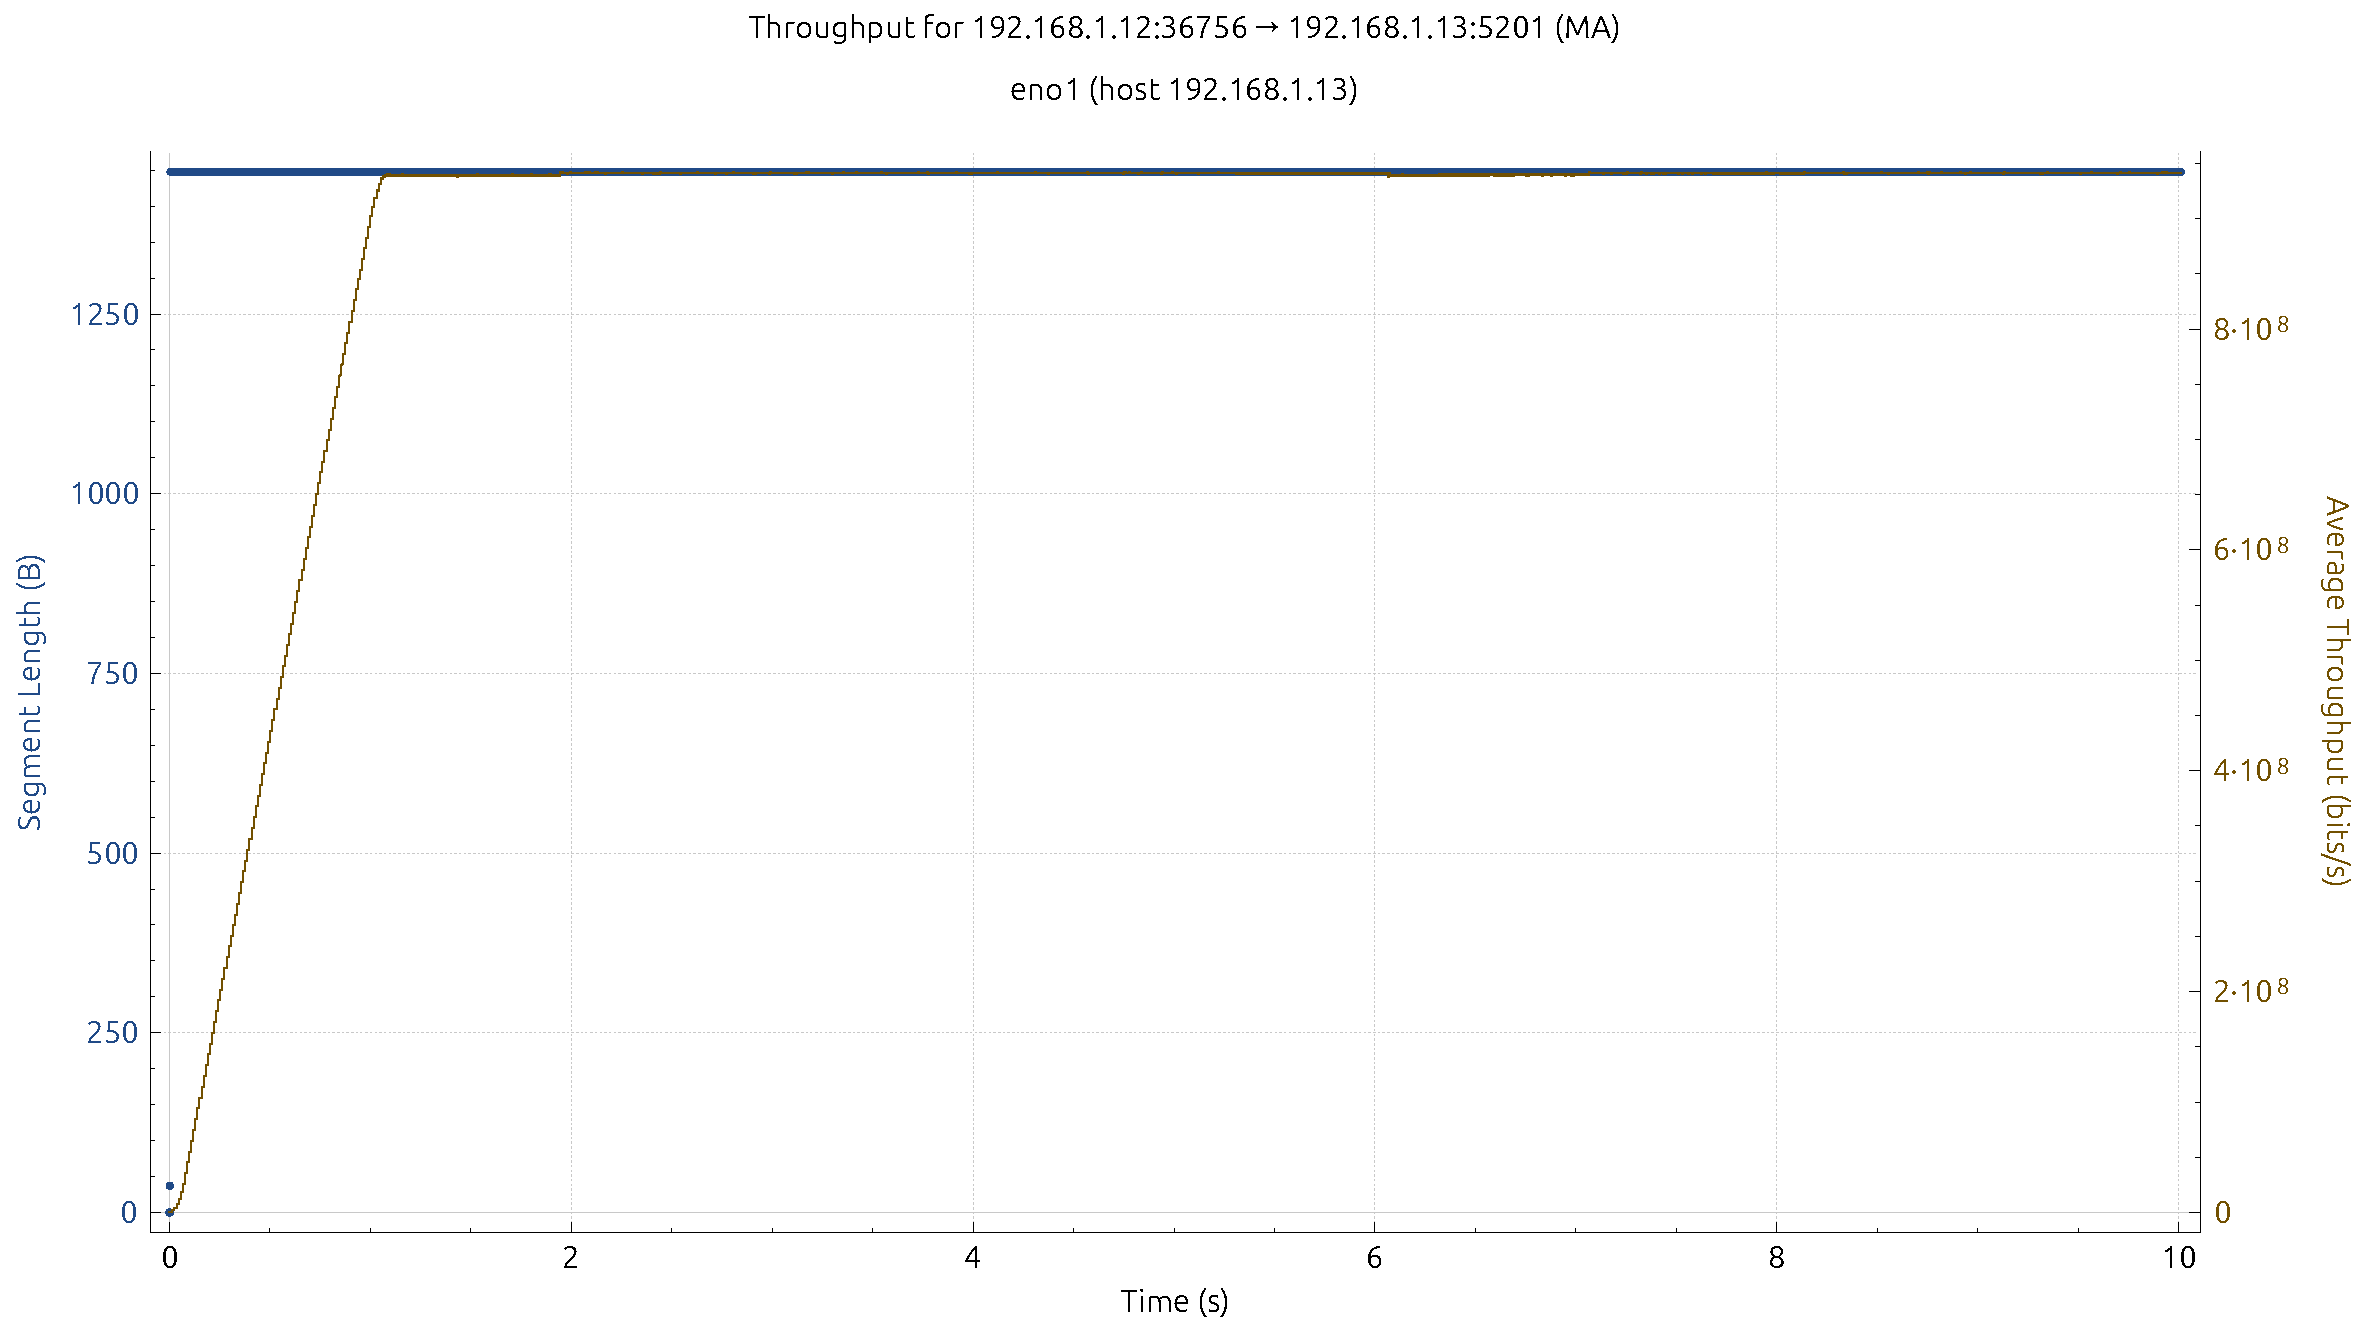
\includegraphics[width=0.9\columnwidth]{images/graphs/Throughput/Throughput_ETH_TCP.pdf}
                    \caption{TCP Throughput in the Ethernet Scenario.}
                    \label{fig:throughput-eth-tcp}
                \end{figure}

                Figure~\ref{fig:rtt-eth-tcp} illustrates the round-trip time (RTT), which remains very low (typically within 1-3 milliseconds), highlighting the minimal latency in wired connections. 
                
                \begin{figure}[ht]
                    \centering
                    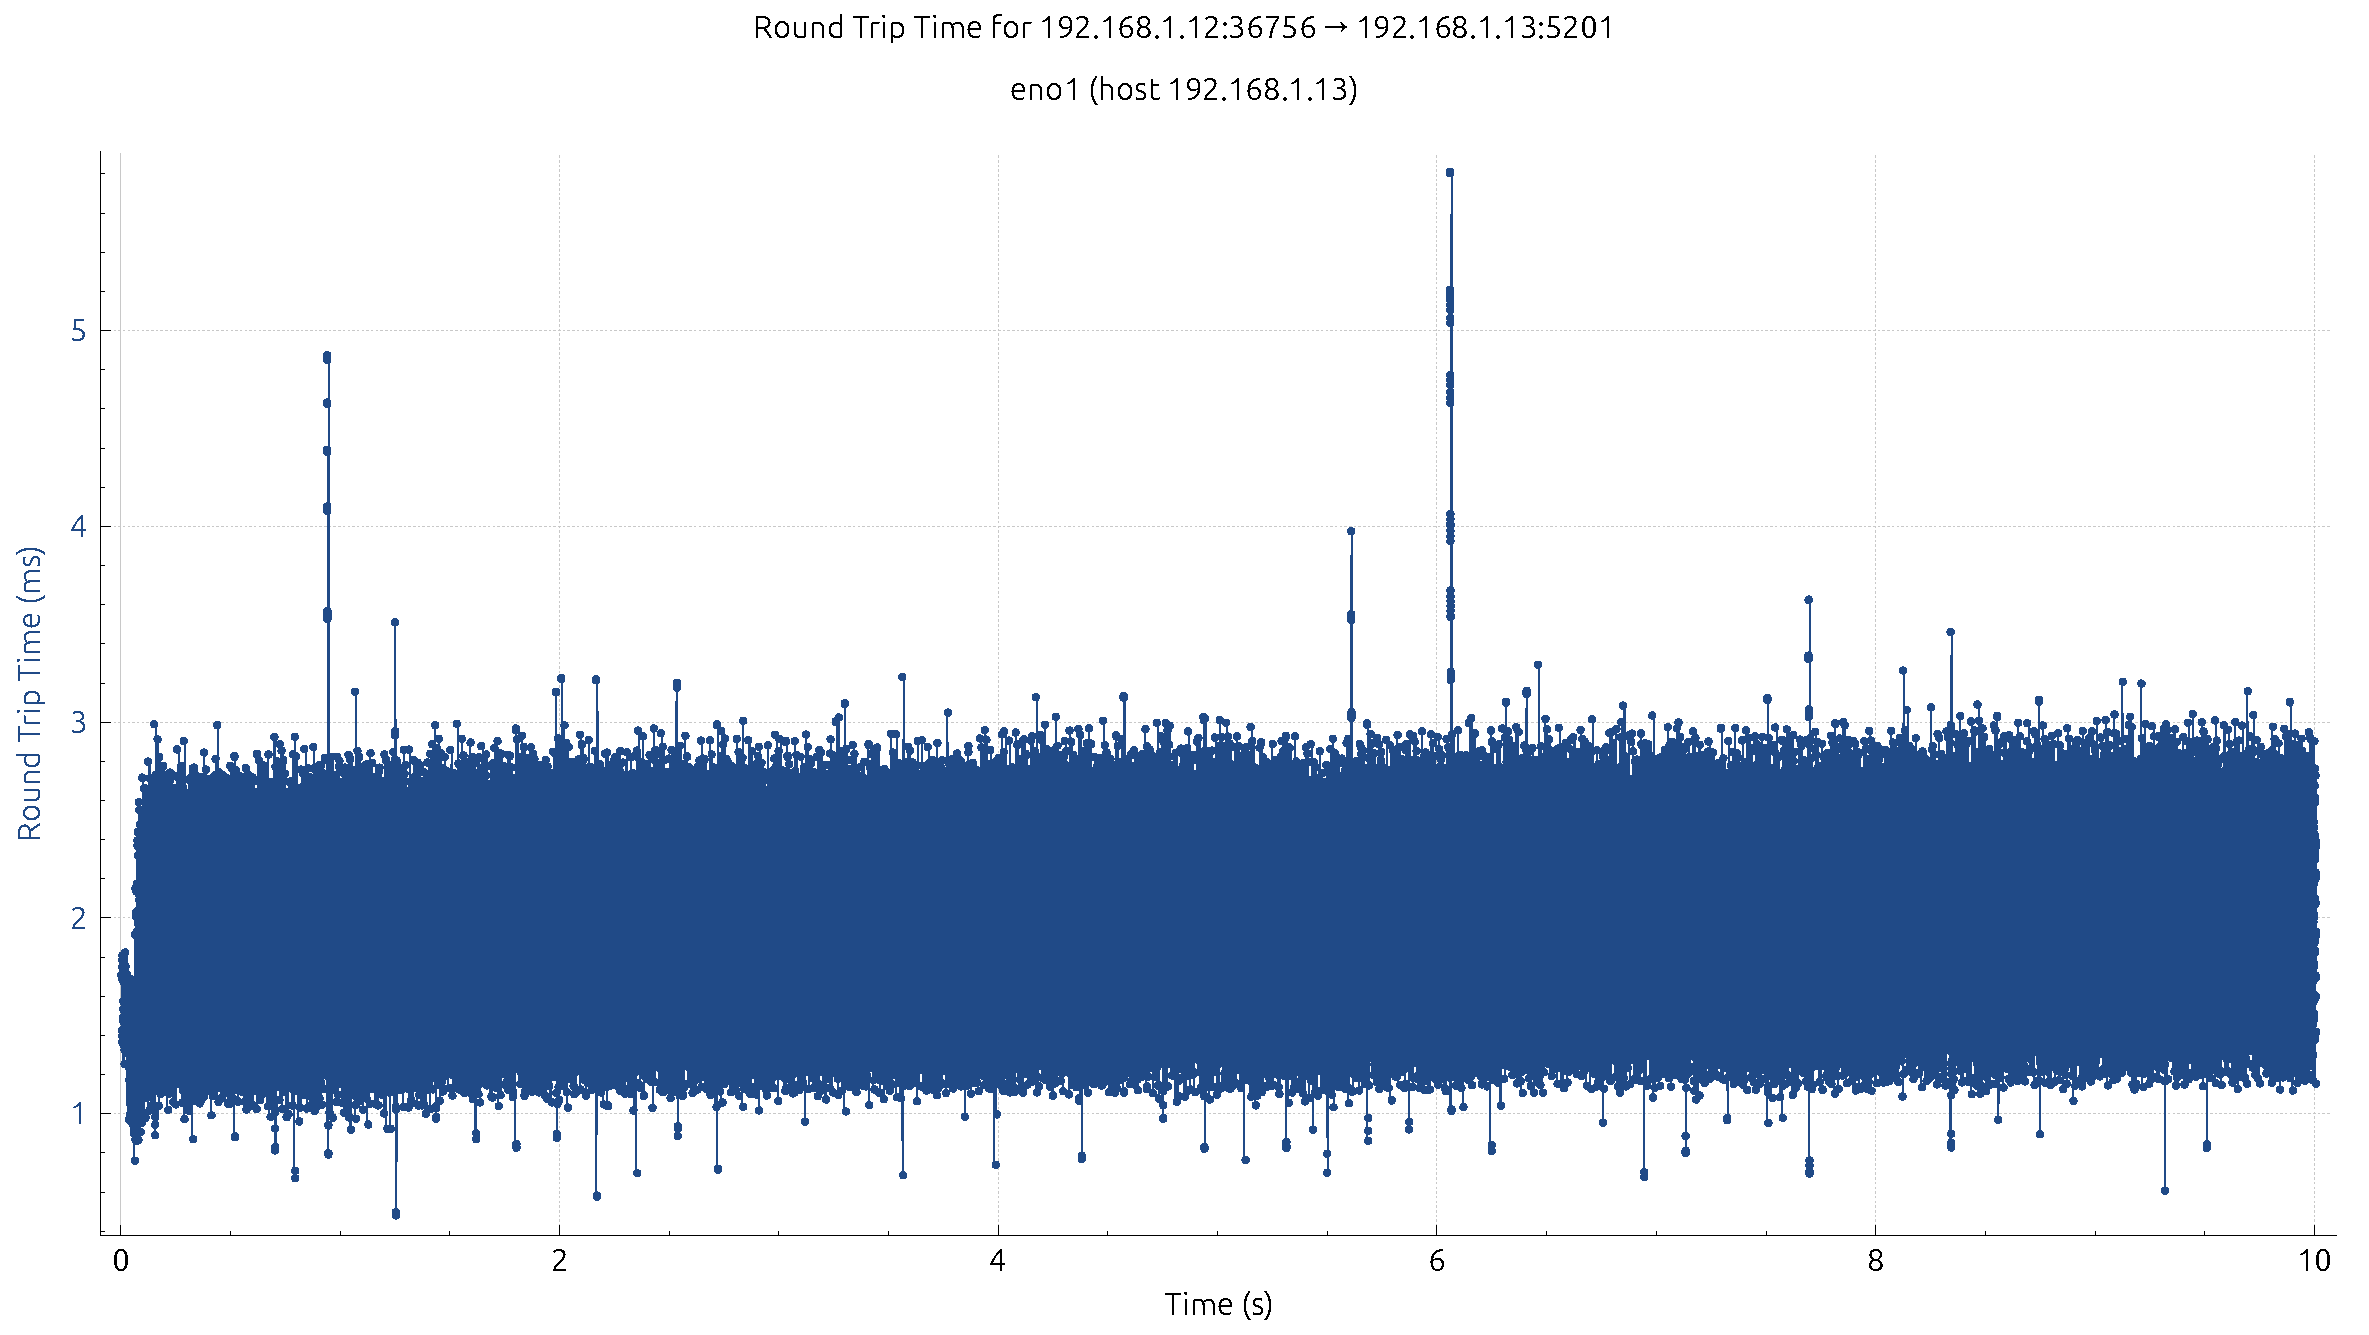
\includegraphics[width=0.9\columnwidth]{images/graphs/RTT/RTT_ETH_TCP.pdf}
                    \caption{TCP Round Trip Time in the Ethernet Scenario.}
                    \label{fig:rtt-eth-tcp}
                \end{figure}

                % Furthermore, the I-O graph (Fig.~\ref{fig:io-eth-tcp}) confirms a consistent packet flow with little variation, indicating that the Ethernet setup effectively utilizes the available capacity. 
                
                % \begin{figure}[ht]
                %     \centering
                %     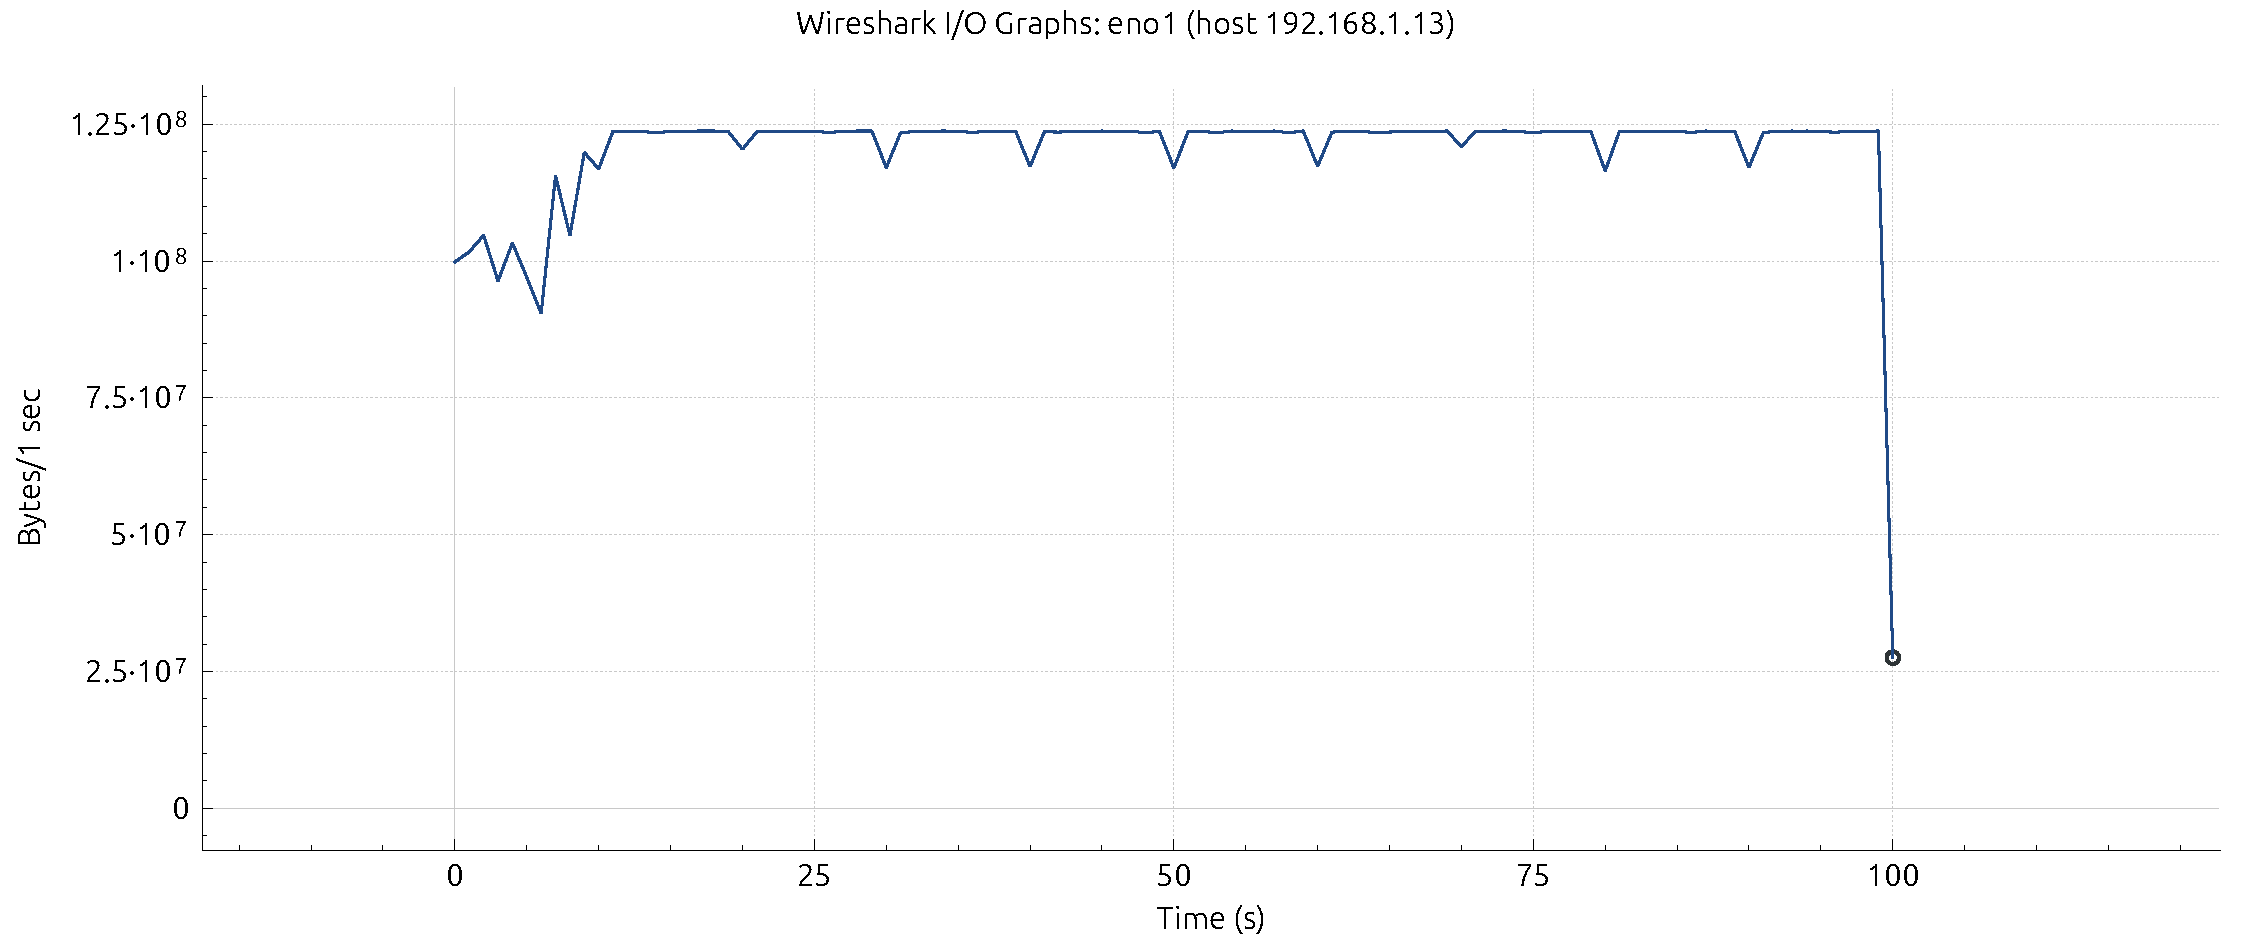
\includegraphics[width=0.9\columnwidth]{images/graphs/I-O/I-O_ETH_TCP.pdf}
                %     \caption{Wireshark I-O Graph for TCP in the Ethernet Scenario.}
                %     \label{fig:io-eth-tcp}
                % \end{figure}

                Overall, the Ethernet scenario demonstrates a near-ideal performance with high throughput and minimal latency, closely matching the theoretical predictions.

            \vspace{0.2cm} % TODO: check

            \item \textbf{Both WiFi:} \\
                In the WiFi trace, the throughput plot (Fig.~\ref{fig:throughput-wifi-tcp}) shows an upfront ramp-up phase over the first 2 seconds, followed by a varying throughput about a mean of 434.7 Mbps. The up and down in these traces due to protocol overhead, some wireless interference, and WiFi being half-duplex, reduces its performing capability.    

                \begin{figure}[ht]
                    \centering
                    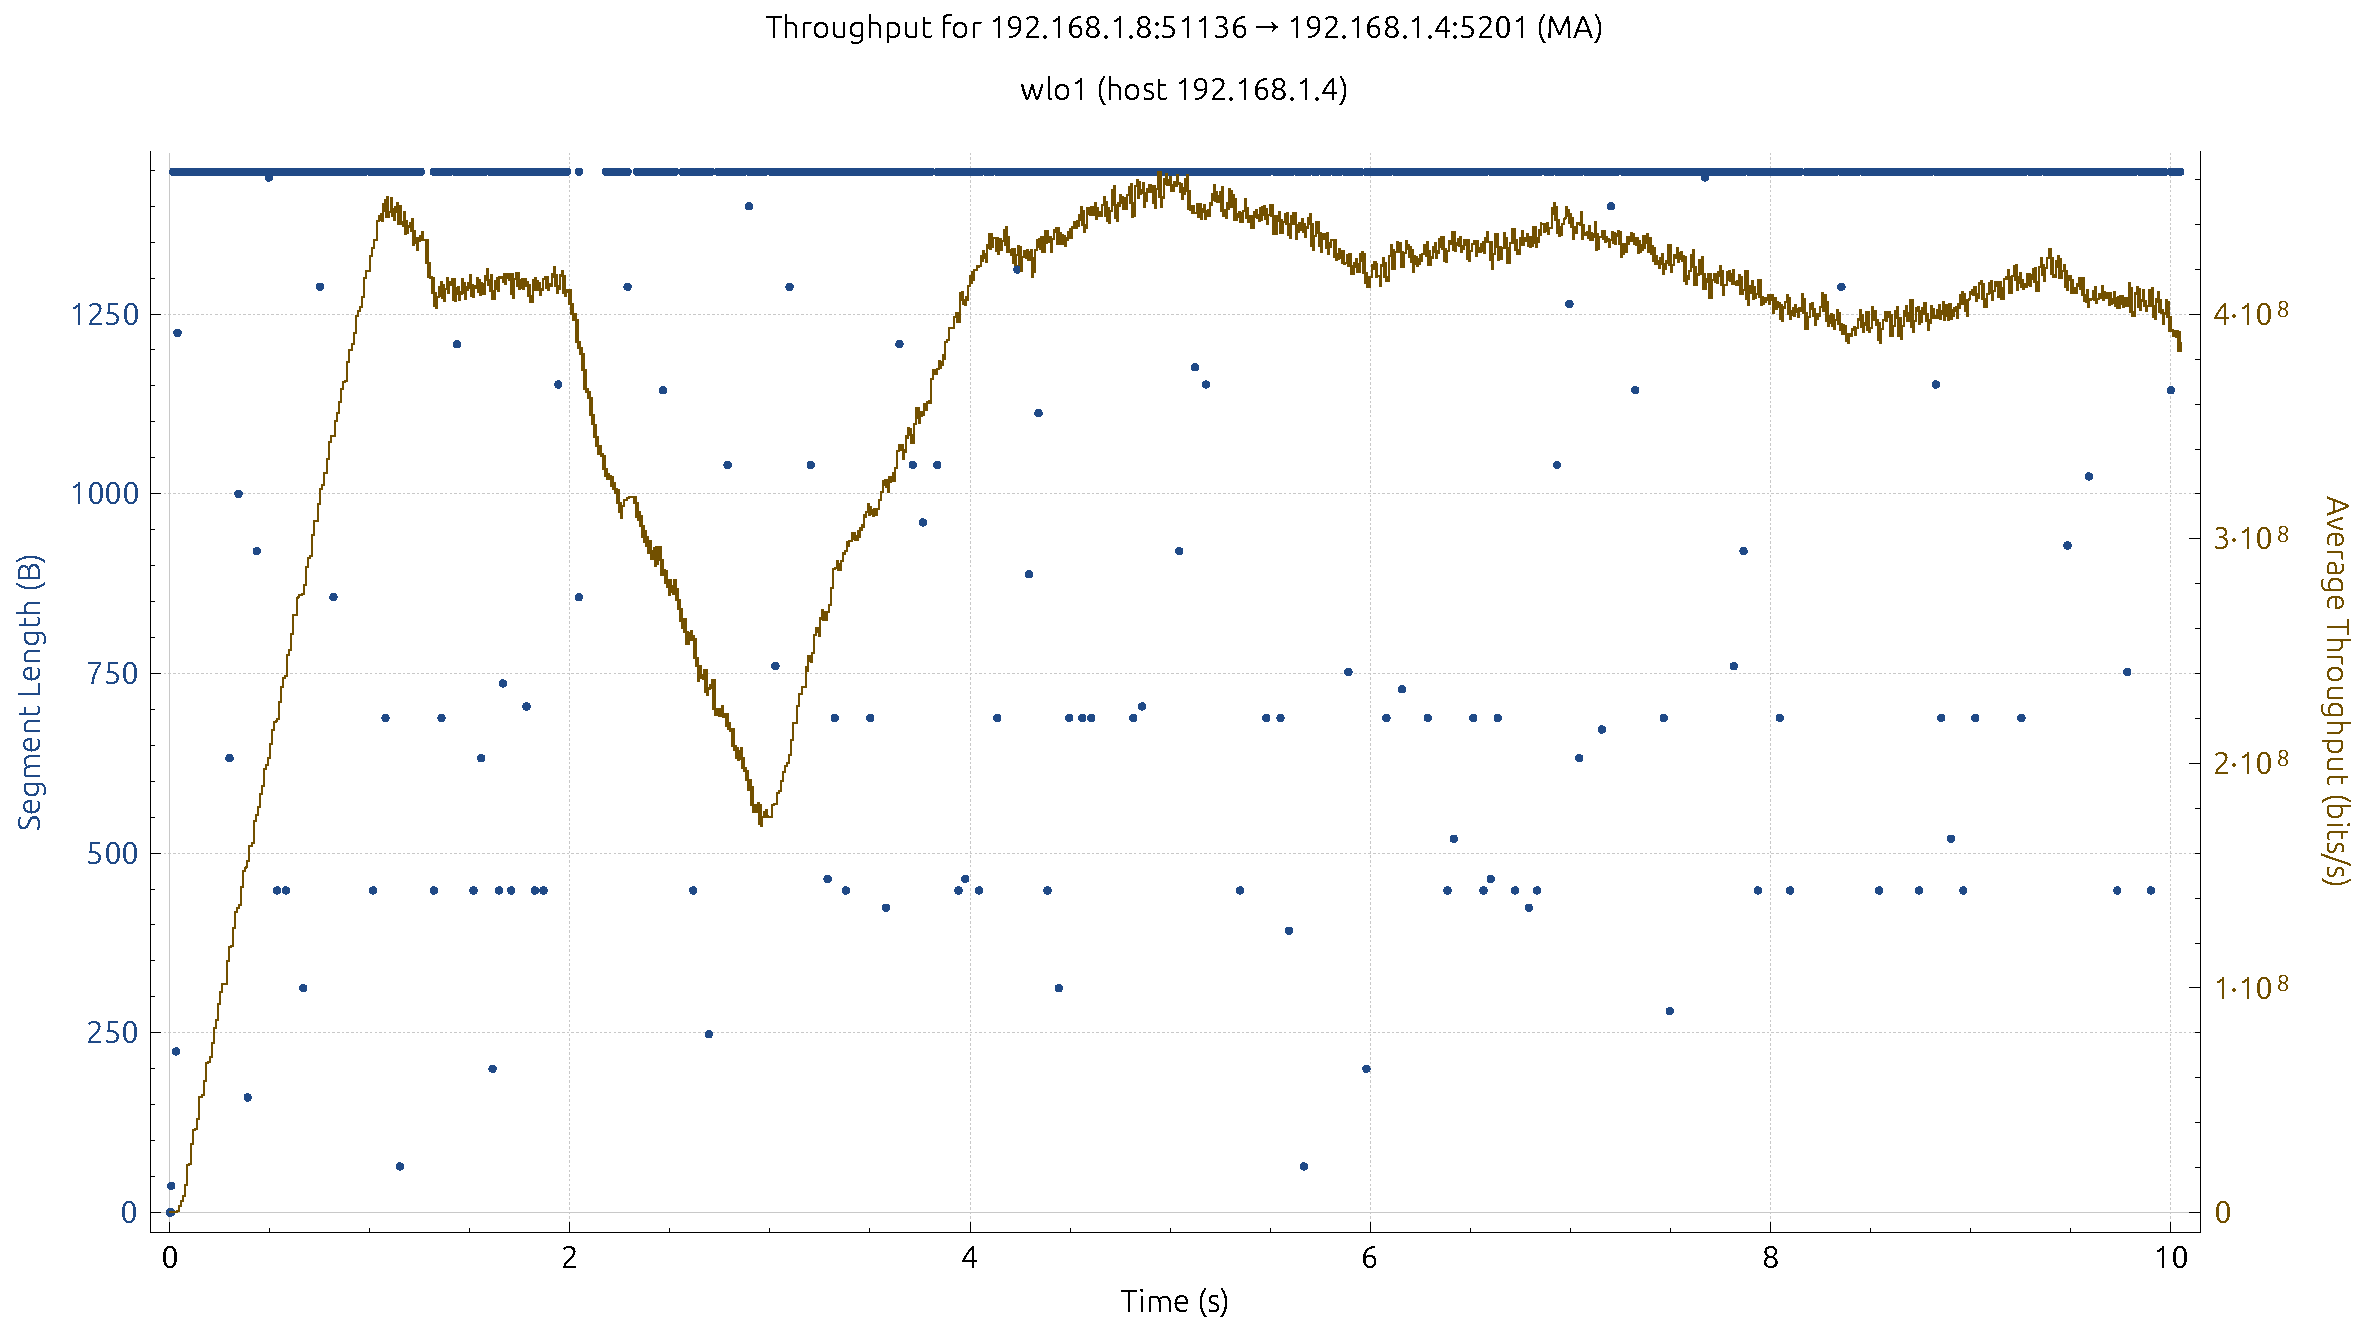
\includegraphics[width=0.9\columnwidth]{images/graphs/Throughput/Throughput_WiFi_TCP.pdf}
                    \caption{TCP Throughput in the WiFi Scenario. \vspace{0.2cm}} % TODO: check
                    \label{fig:throughput-wifi-tcp}
                \end{figure}

                RTT measurements (Fig. 4) show RTT in the range of around 20-50 ms, with some delays probably caused by congestion and contention in the wireless medium.
                
                \begin{figure}[ht]
                    \centering
                    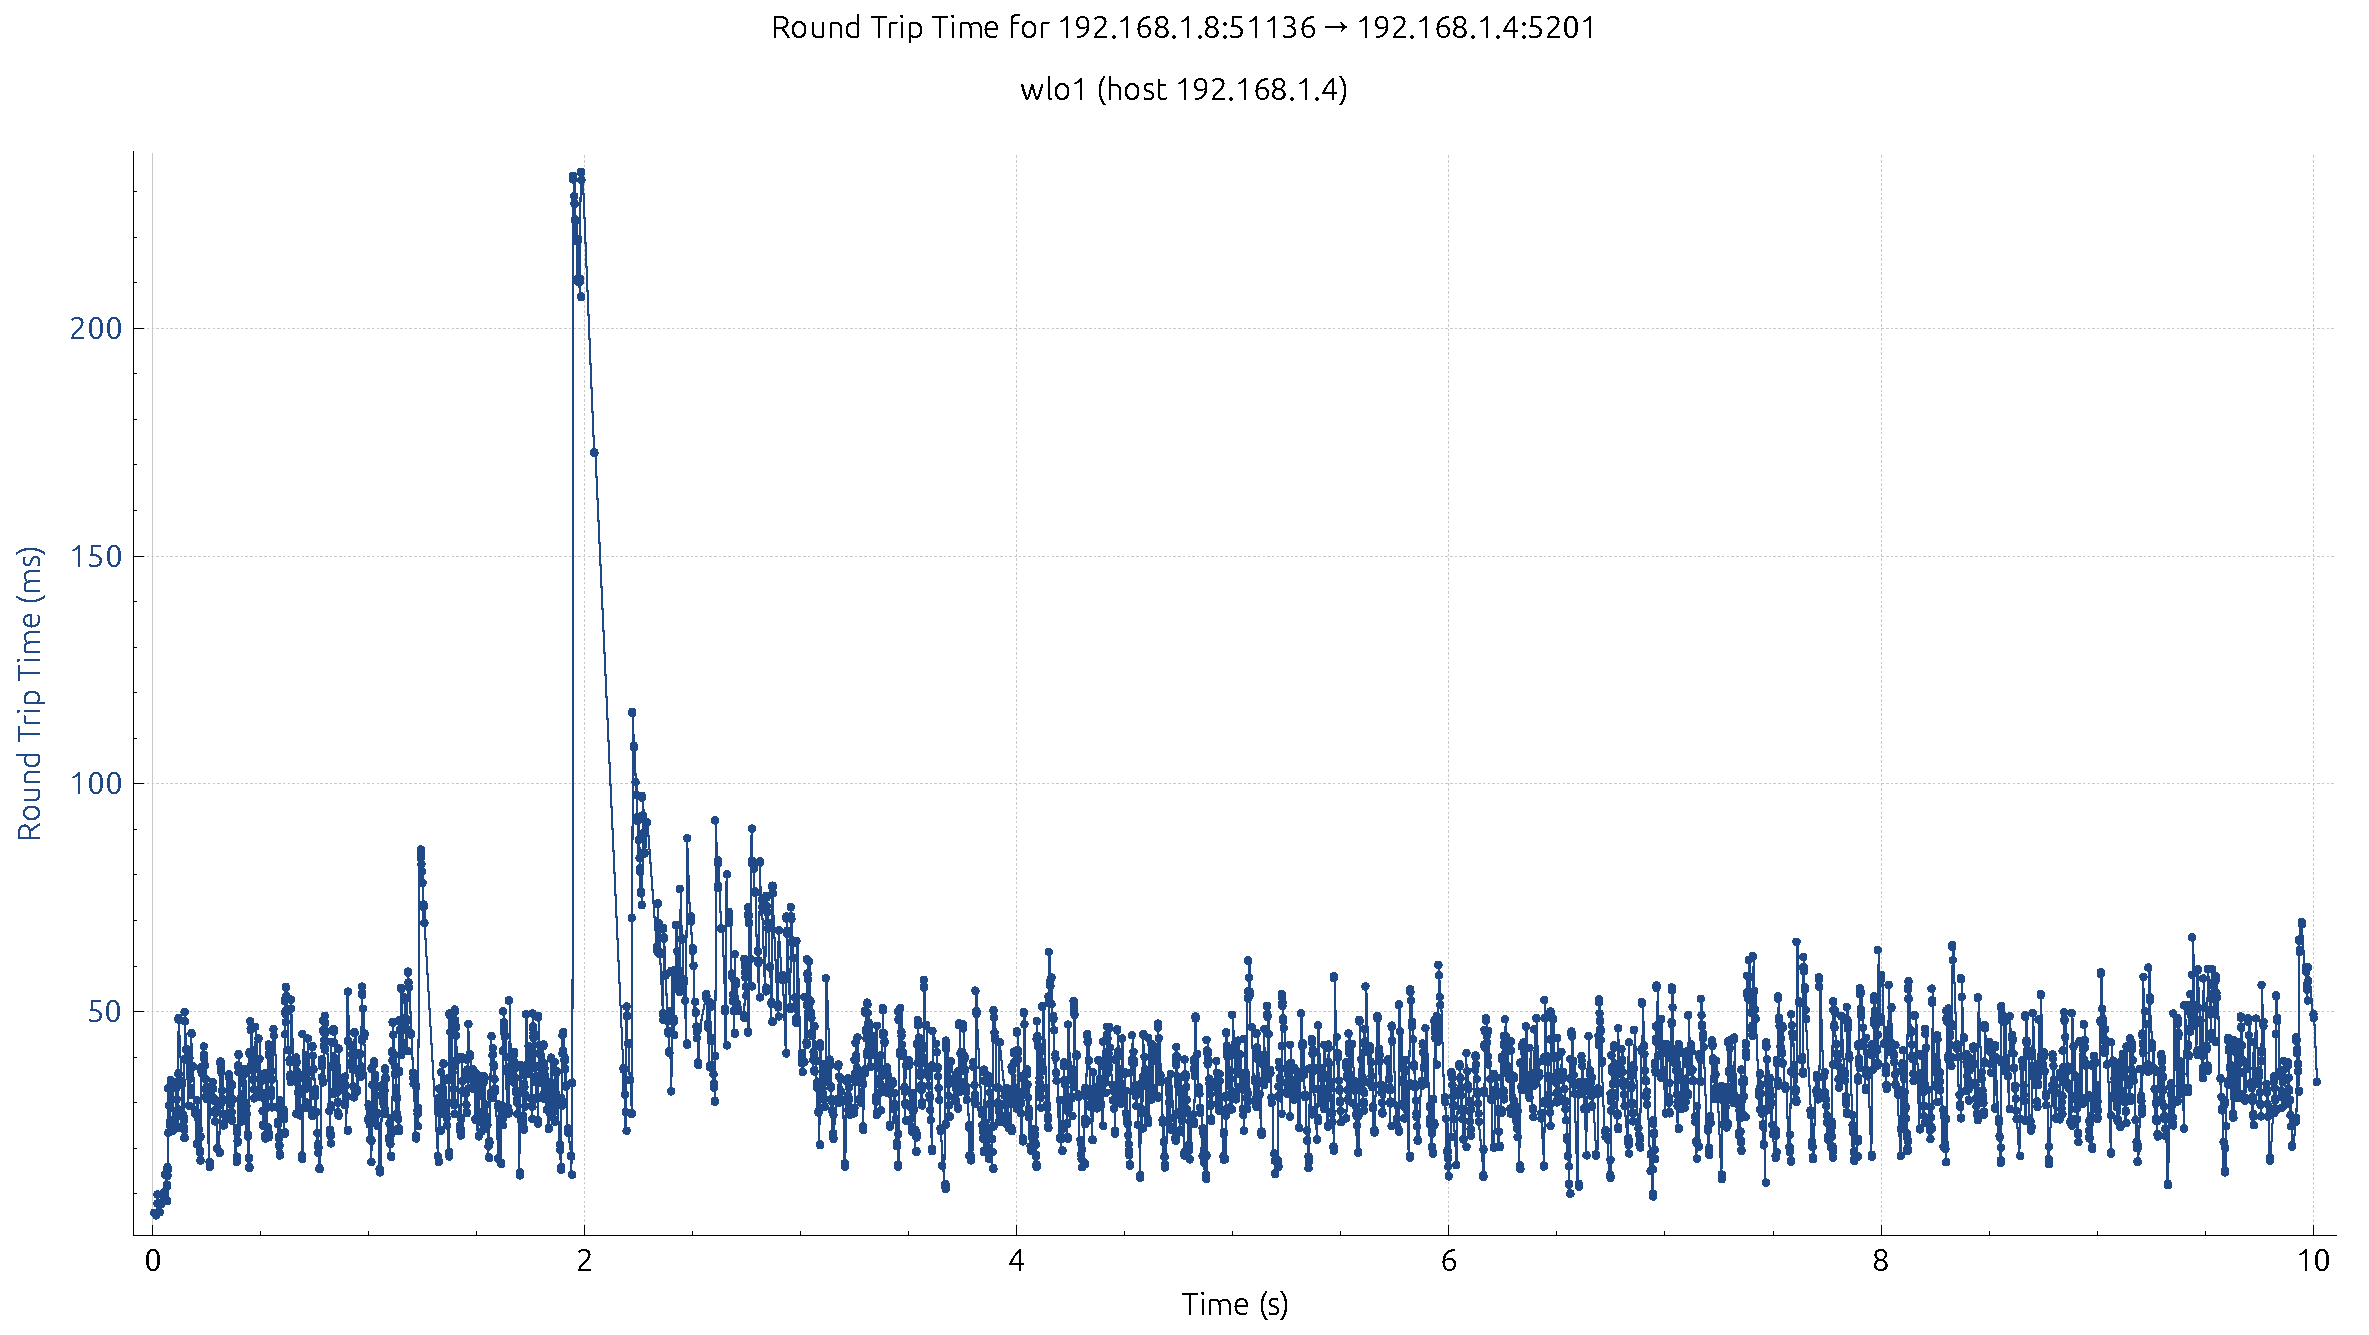
\includegraphics[width=0.9\columnwidth]{images/graphs/RTT/RTT_WiFi_TCP.pdf}
                    \caption{TCP Round Trip Time in the WiFi Scenario.}
                    \label{fig:rtt-wifi-tcp}
                \end{figure}    

                % Furthermore, the I-O graph (Fig.~\ref{fig:io-wifi-tcp}) illustrates a variable number of transmitted packets per interval, reflecting the dynamic nature of WiFi communication where channel conditions and collision avoidance mechanisms influence performance.
                
                % \begin{figure}[ht]
                %     \centering
                %     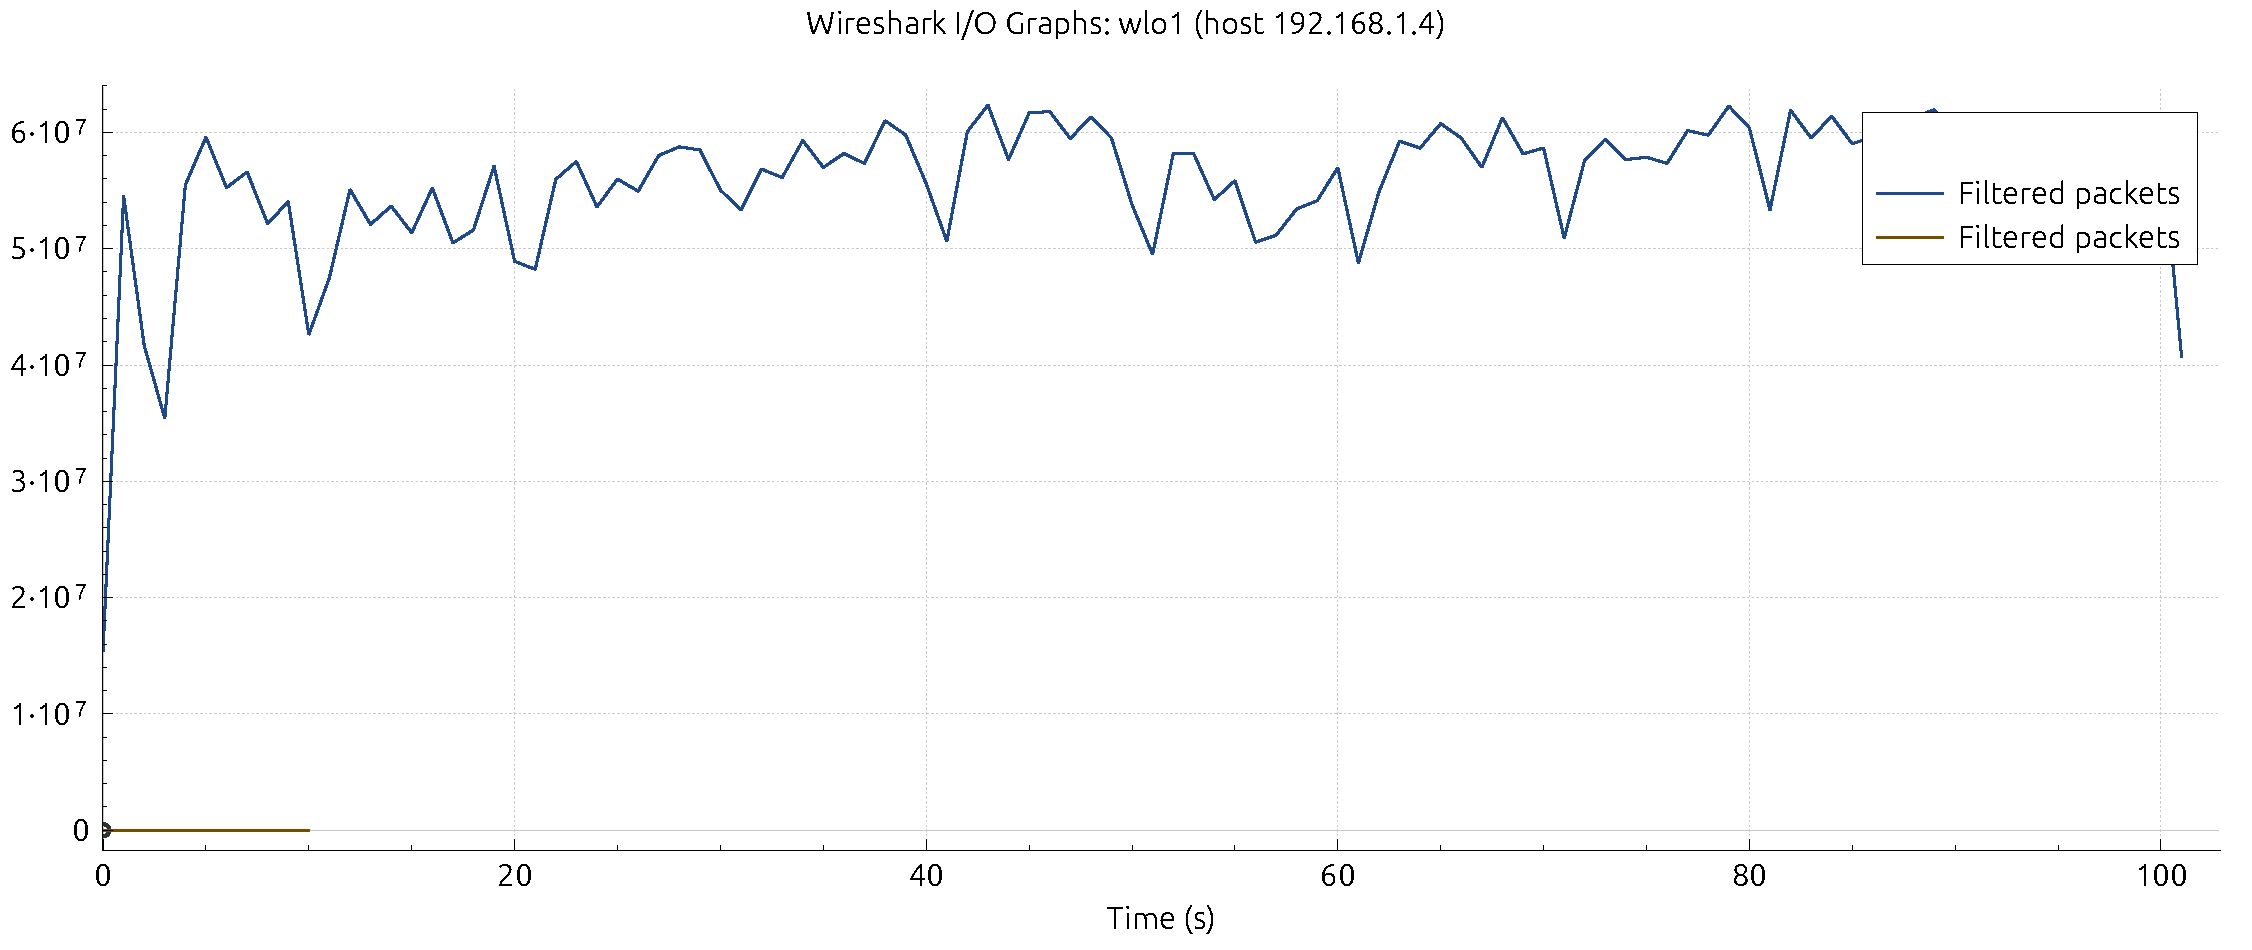
\includegraphics[width=0.9\columnwidth]{images/graphs/I-O/I-O_WiFi_TCP.pdf}
                %     \caption{Wireshark I-O Graph for TCP in the WiFi Scenario.}
                %     \label{fig:io-wifi-tcp}
                % \end{figure}}

                Overall, while the theoretical limit for TCP over WiFi is approximated to around 480 Mbps, experimental observation indicates that real-world factors does not reduce so significantly the effective throughput of the WiFi network. This as the network was in a state of perfection, where there was just the server and client that were connected to the access point and no other computers were generating traffic.

            \vspace{0.2cm} % TODO: check

            \item \textbf{Mixed:} \\
                Figure~\ref{fig:throughput-mix-tcp} displays the TCP throughput for the mixed configuration. 
                While the theoretical model identifies Ethernet as the bottleneck, experimental results reveal the wireless segment’s critical impact. The graph shows that the throughput reaches a stable level after an initial ramp-up phase, although it remains below the Ethernet scenario and is consistent with the expected reduction due to the reliance on the wireless link.

                \begin{figure}[ht]
                    \centering
                    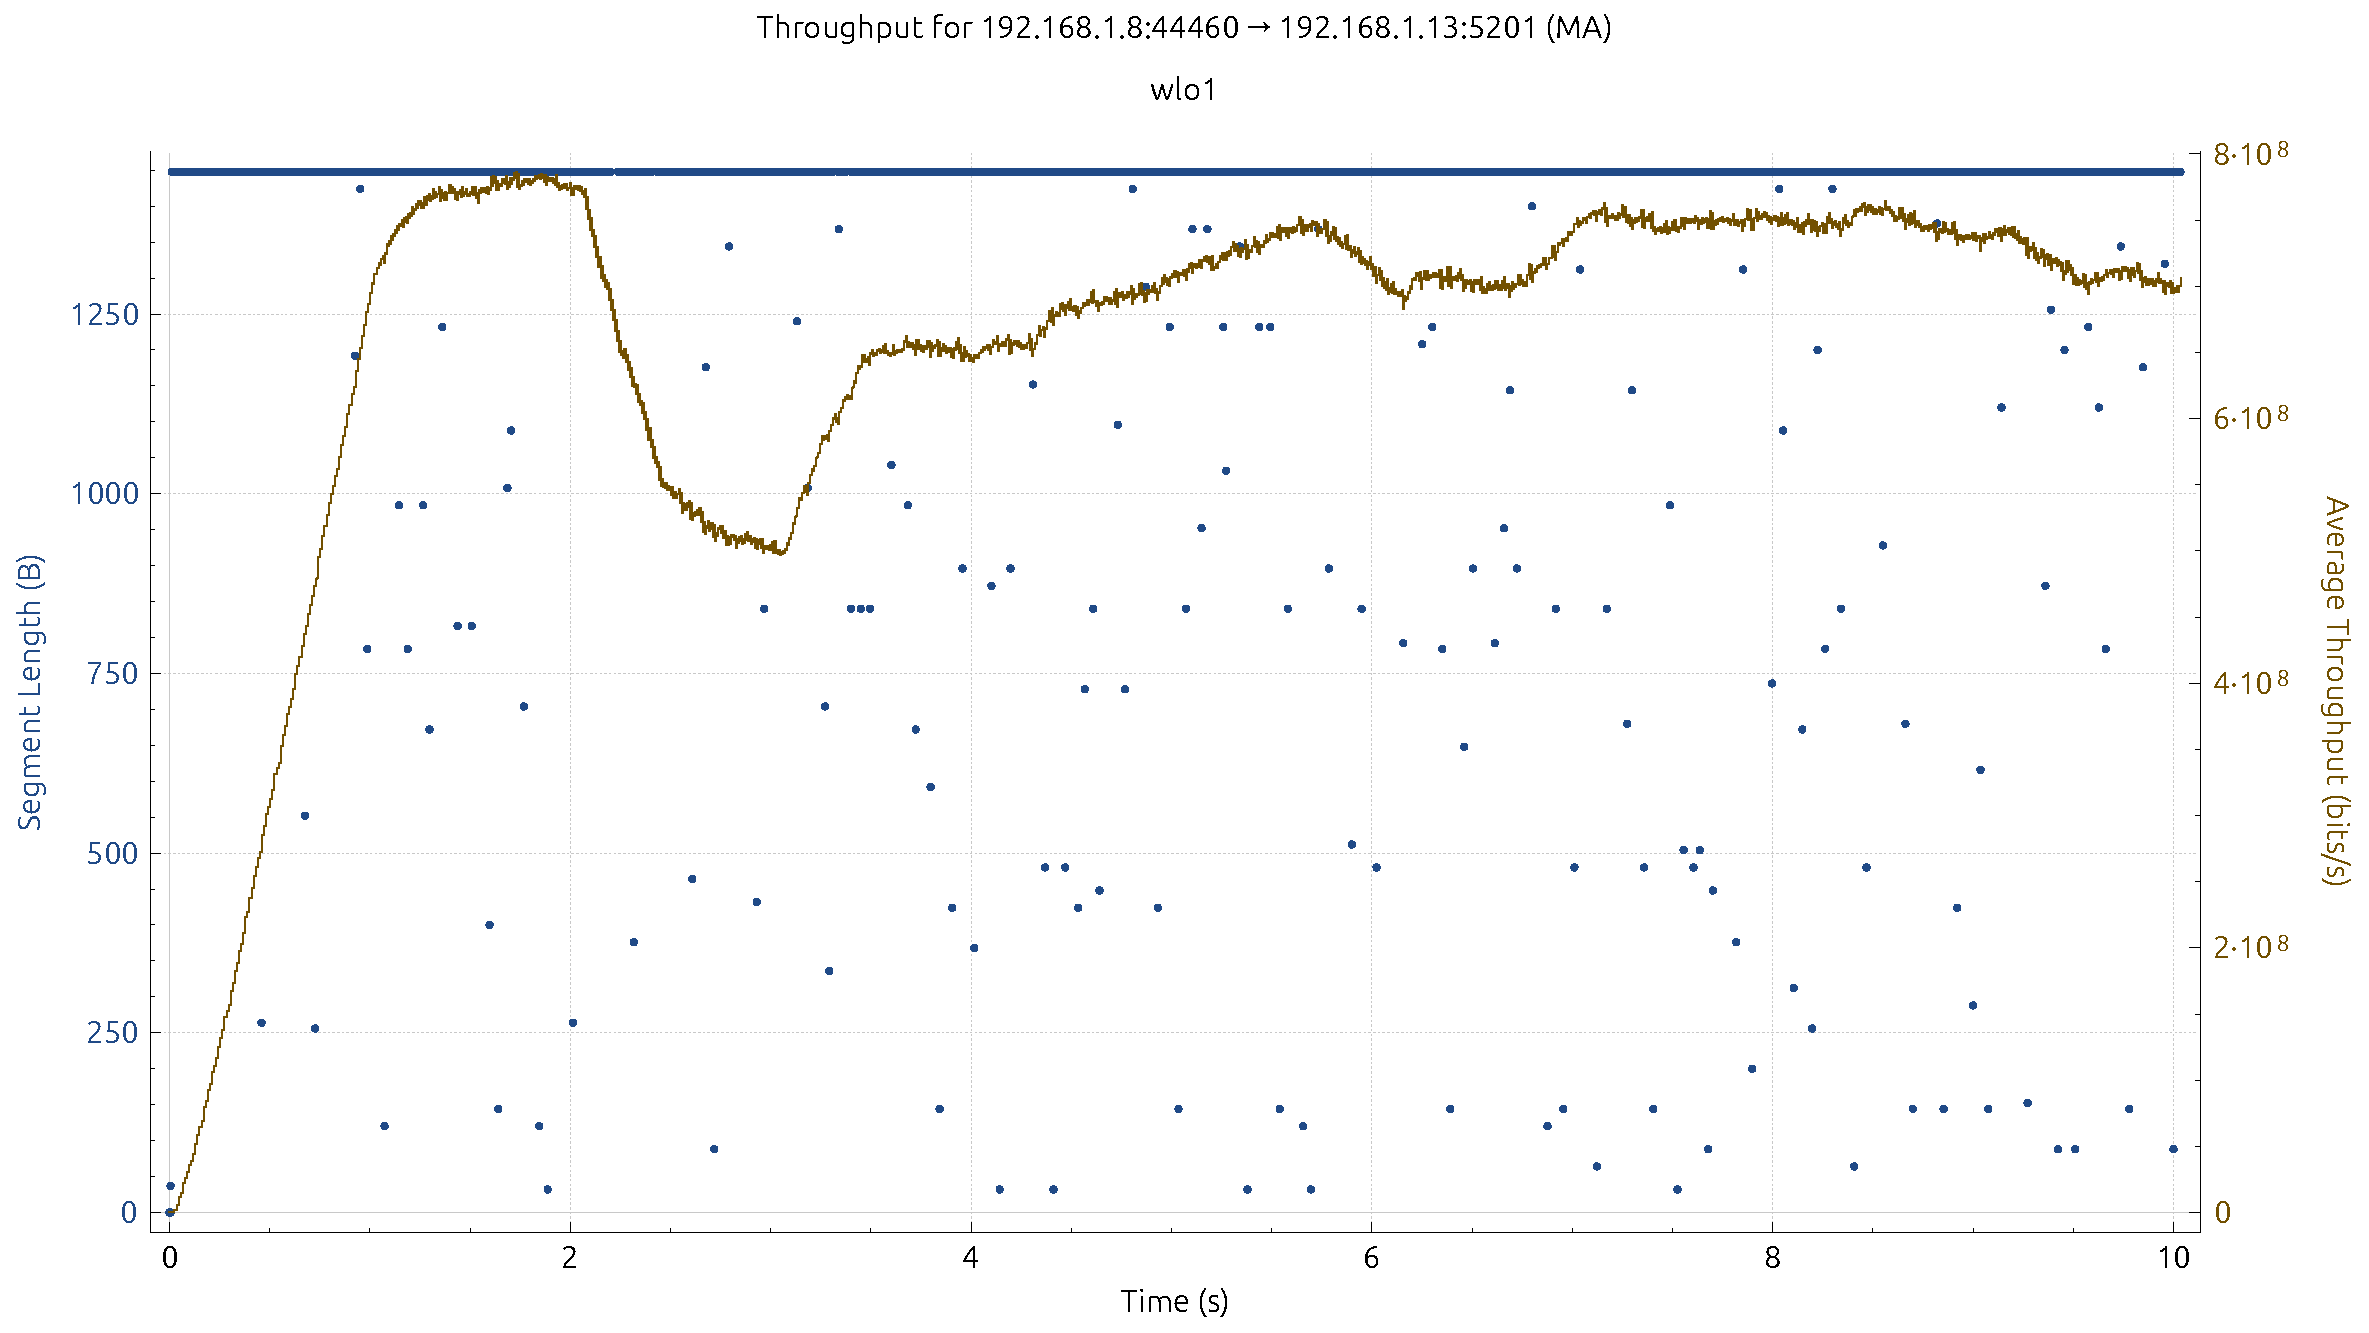
\includegraphics[width=0.9\columnwidth]{images/graphs/Throughput/Throughput_MIX_TCP.pdf}
                    \caption{TCP Throughput in the Mixed Ethernet/WiFi Scenario.}
                    \label{fig:throughput-mix-tcp}
                \end{figure}

                The round-trip time (RTT) measurements in Figure~\ref{fig:rtt-mix-tcp} directly explain TCP’s throughput limitations: the protocol adapts its congestion window based on RTT, and the stark latency disparity between Ethernet (1–3 ms) and WiFi (20–50 ms) triggers overly conservative adjustments, capping throughput far below theoretical predictions.

                \begin{figure}[ht]
                    \centering
                    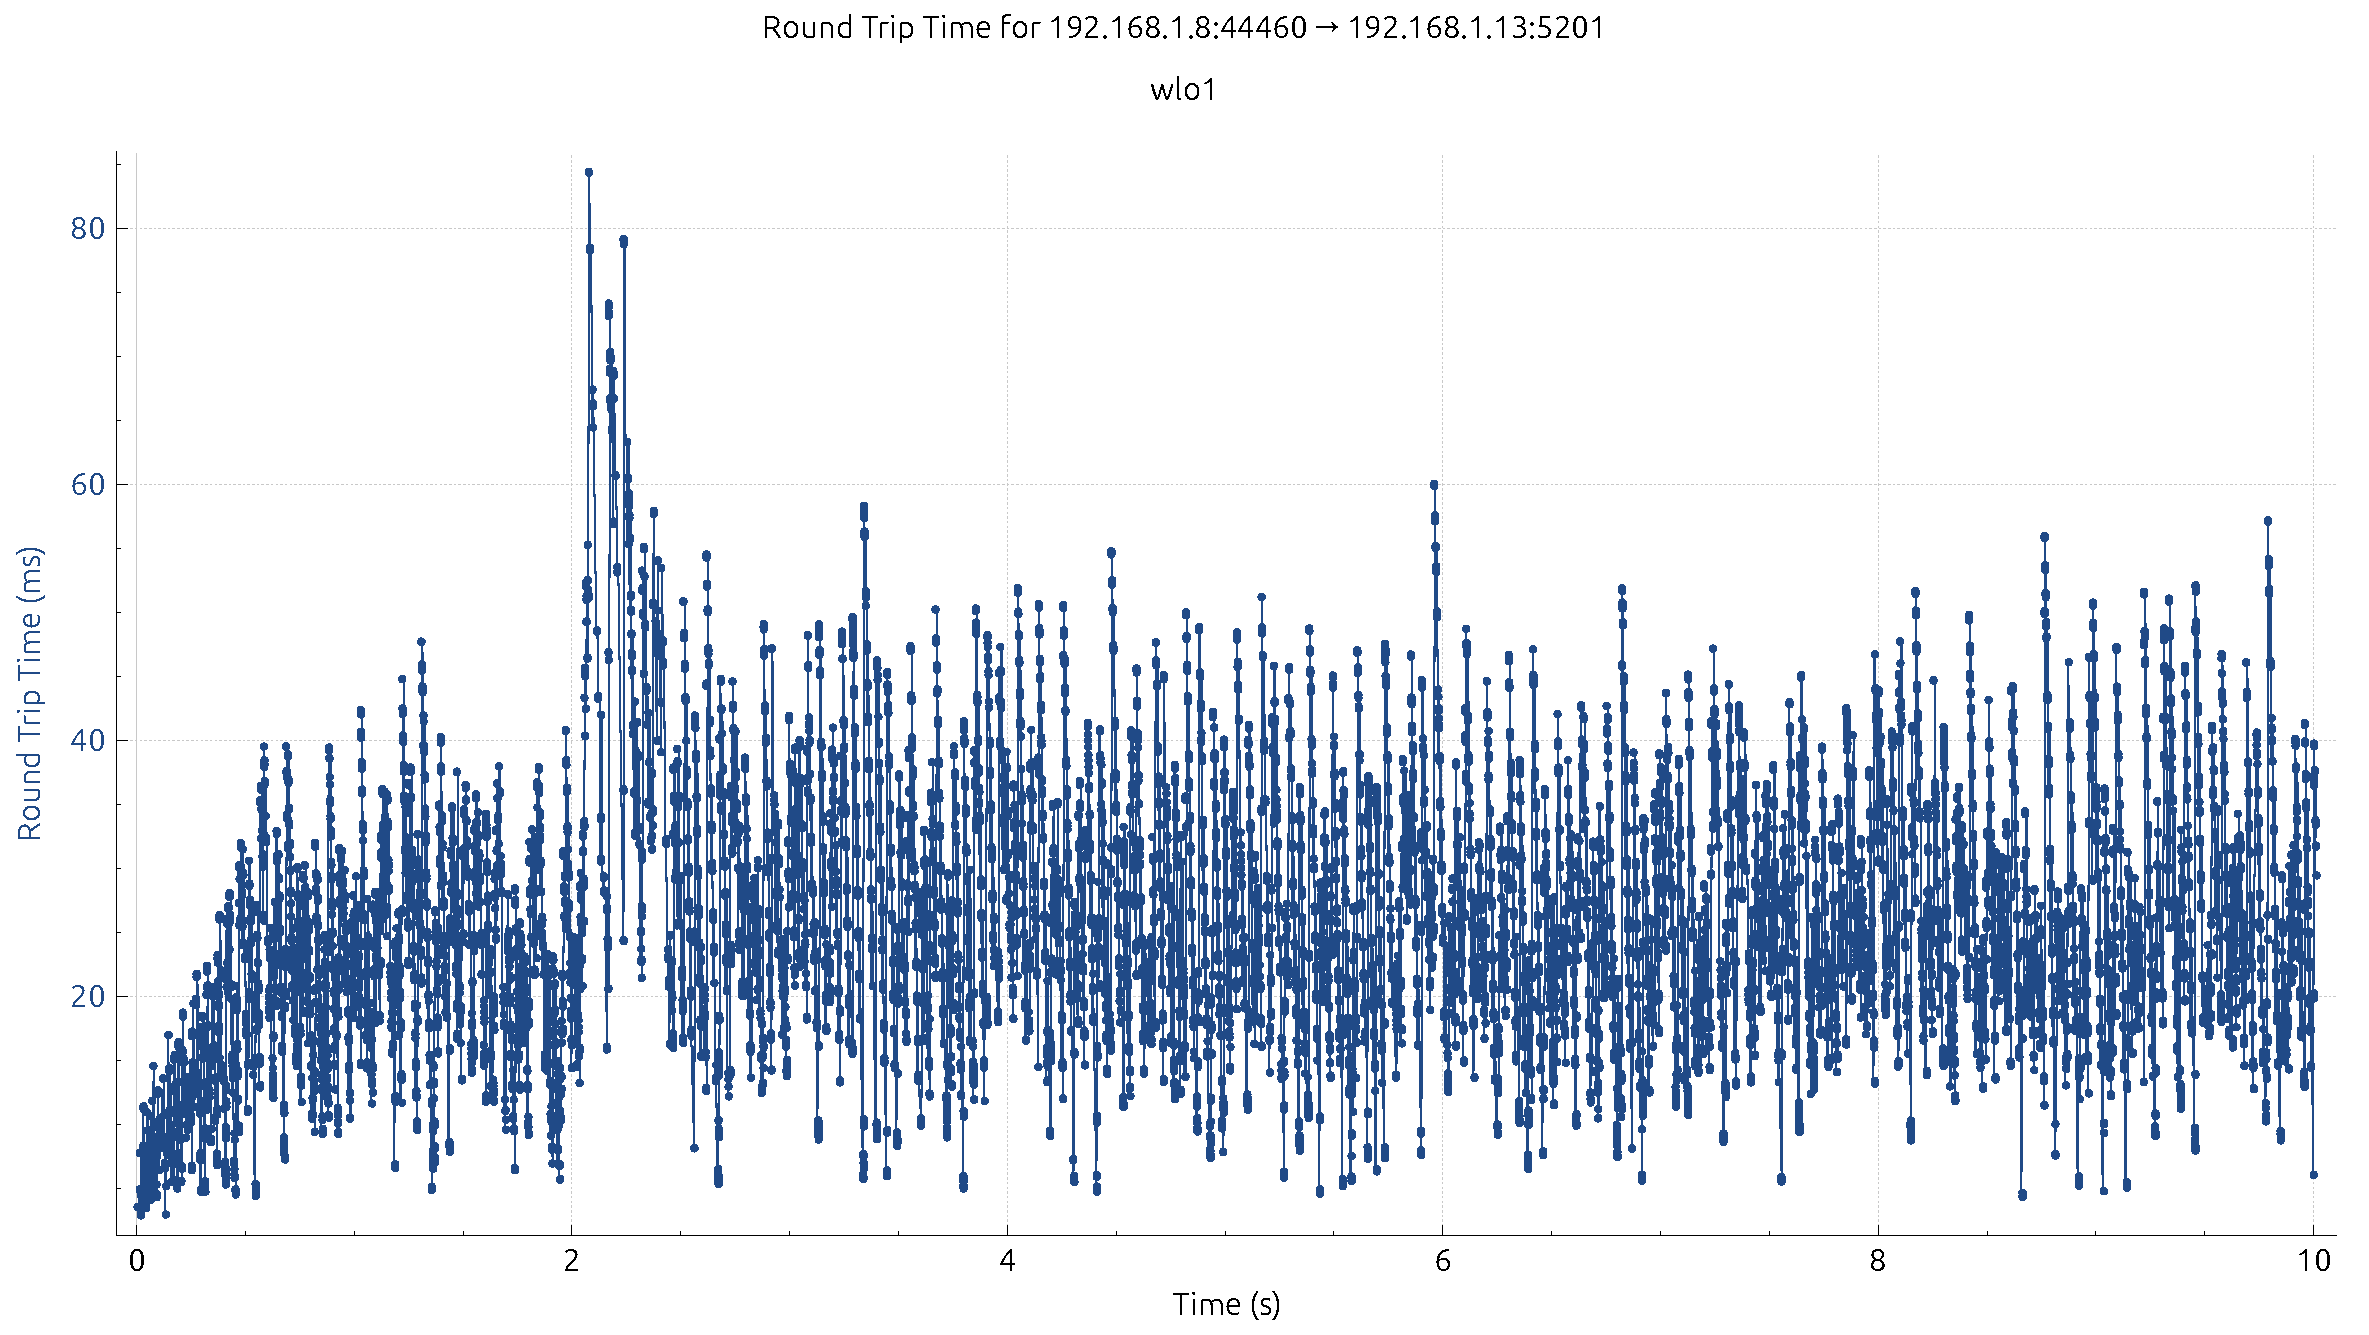
\includegraphics[width=0.9\columnwidth]{images/graphs/RTT/RTT_MIX_TCP.pdf}
                    \caption{TCP Round Trip Time in the Mixed Ethernet/WiFi Scenario.}
                    \label{fig:rtt-mix-tcp}
                \end{figure}

                % The I-O graph for TCP (Fig.~\ref{fig:io-mix-tcp}) shows a relatively steady packet flow over the test intervals, confirming that the mixed configuration maintains a stable performance despite the inherent variability of the wireless link.

                % \begin{figure}[ht]
                %     \centering
                %     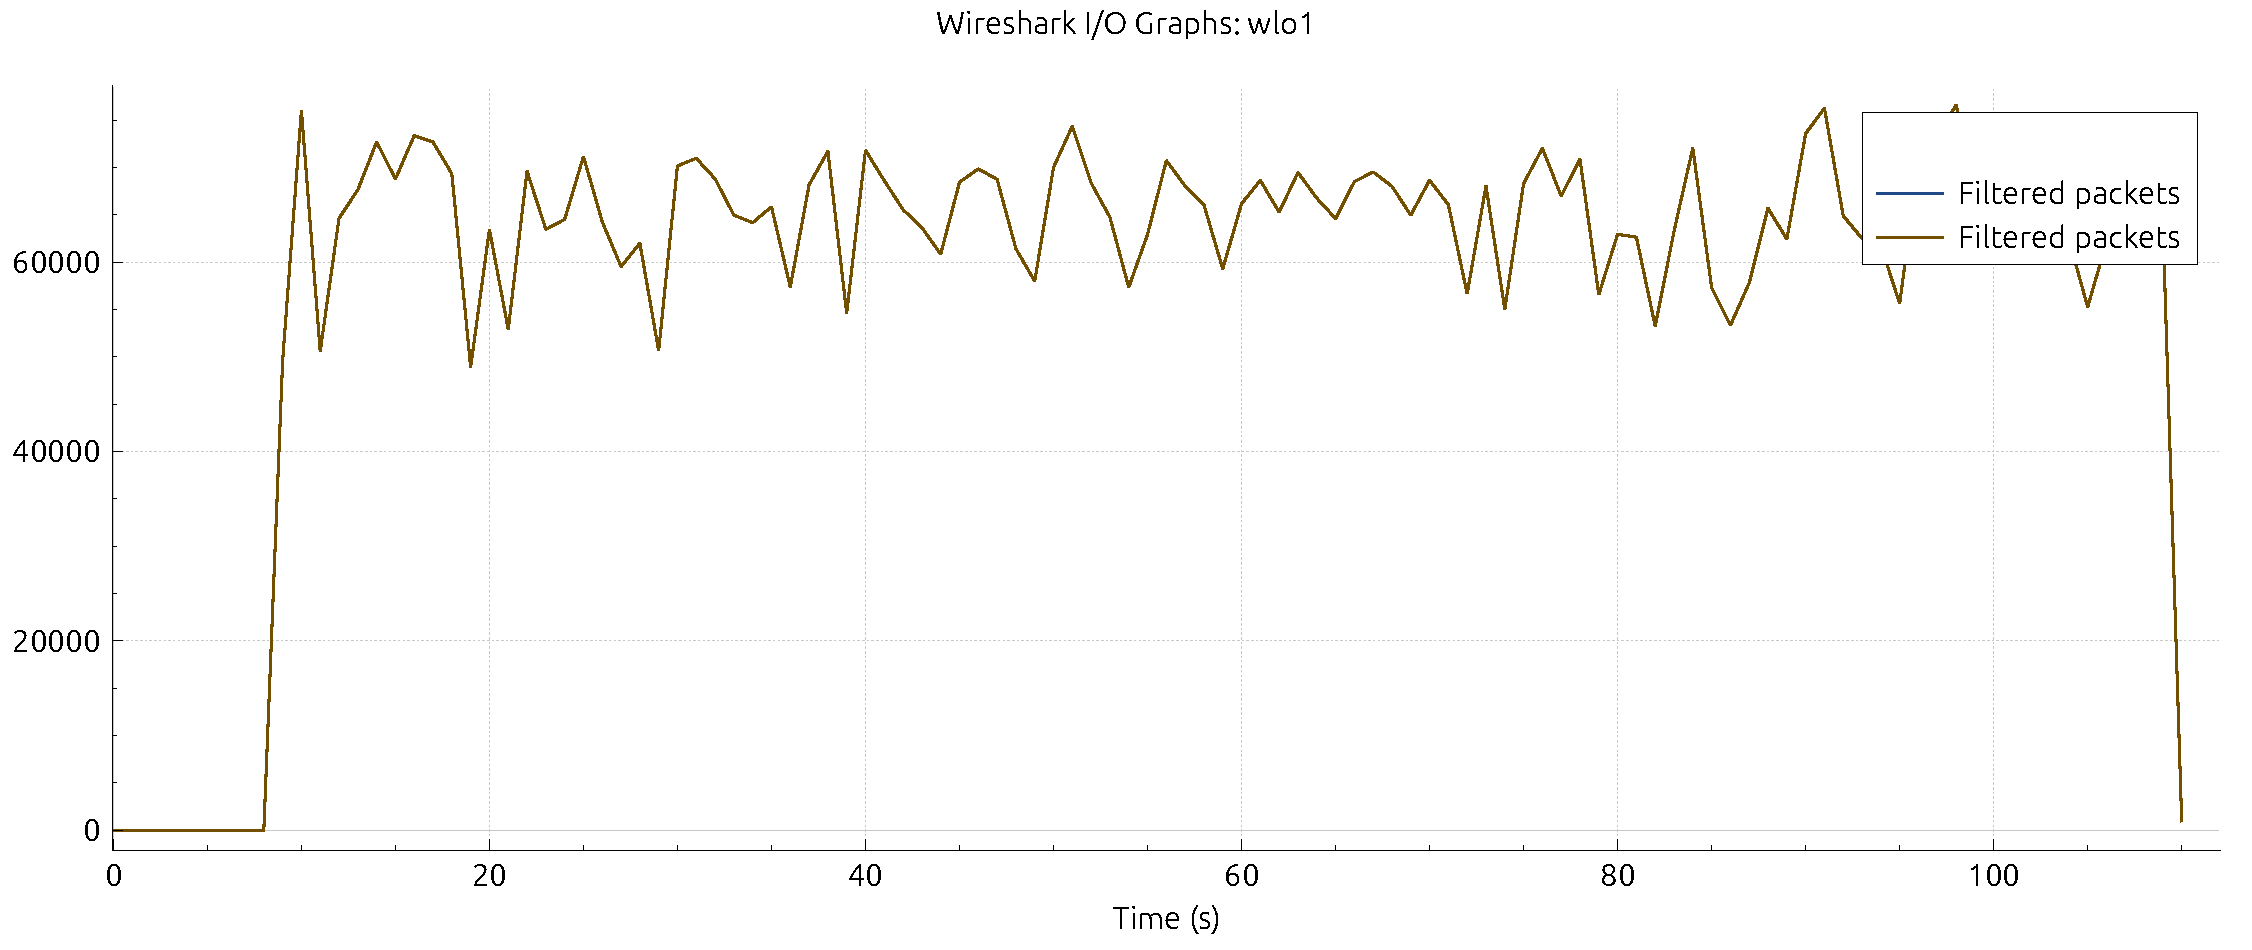
\includegraphics[width=0.9\columnwidth]{images/graphs/I-O/I-O_MIX_TCP.pdf}
                %     \caption{Wireshark I-O Graph for TCP in the Mixed Scenario.}
                %     \label{fig:io-mix-tcp}
                % \end{figure}

            \vspace{0.2cm} % TODO: check
                
            \item[3a.] \textbf{Shared Capacity:} \\
                In this scenario, a third host connected to the same access point was concurrently downloading the film "Natale a Rio"~\cite{Natale_a_Rio} (directed by Neri Parenti), which introduced significant interference during the tests. 
                This additional traffic compromised the available network capacity, leading to degraded performance.
                % Figure~\ref{fig:throughput-mitm-tcp} shows the TCP throughput under this shared capacity condition. 
                % Compared to the mixed scenario without interference, the throughput exhibits a notable decrease. 
                As we can see in (Fig.~\ref{fig:io-mitm-tcp}), the other host starts the download from the second test (\textasciitilde25 seconds). In fact the value of the throughtput, goes from the one of the standard Mixed Scenario (\textbf{\textasciitilde670Mbps}), to a lower one (\textbf{\textasciitilde500Mbps}),
                This behavior is due to the fact that the bandwidth is shared between the two hosts, and the download of the movie is consuming useful bandwidth.

                % \begin{figure}[ht]
                %     \centering
                %     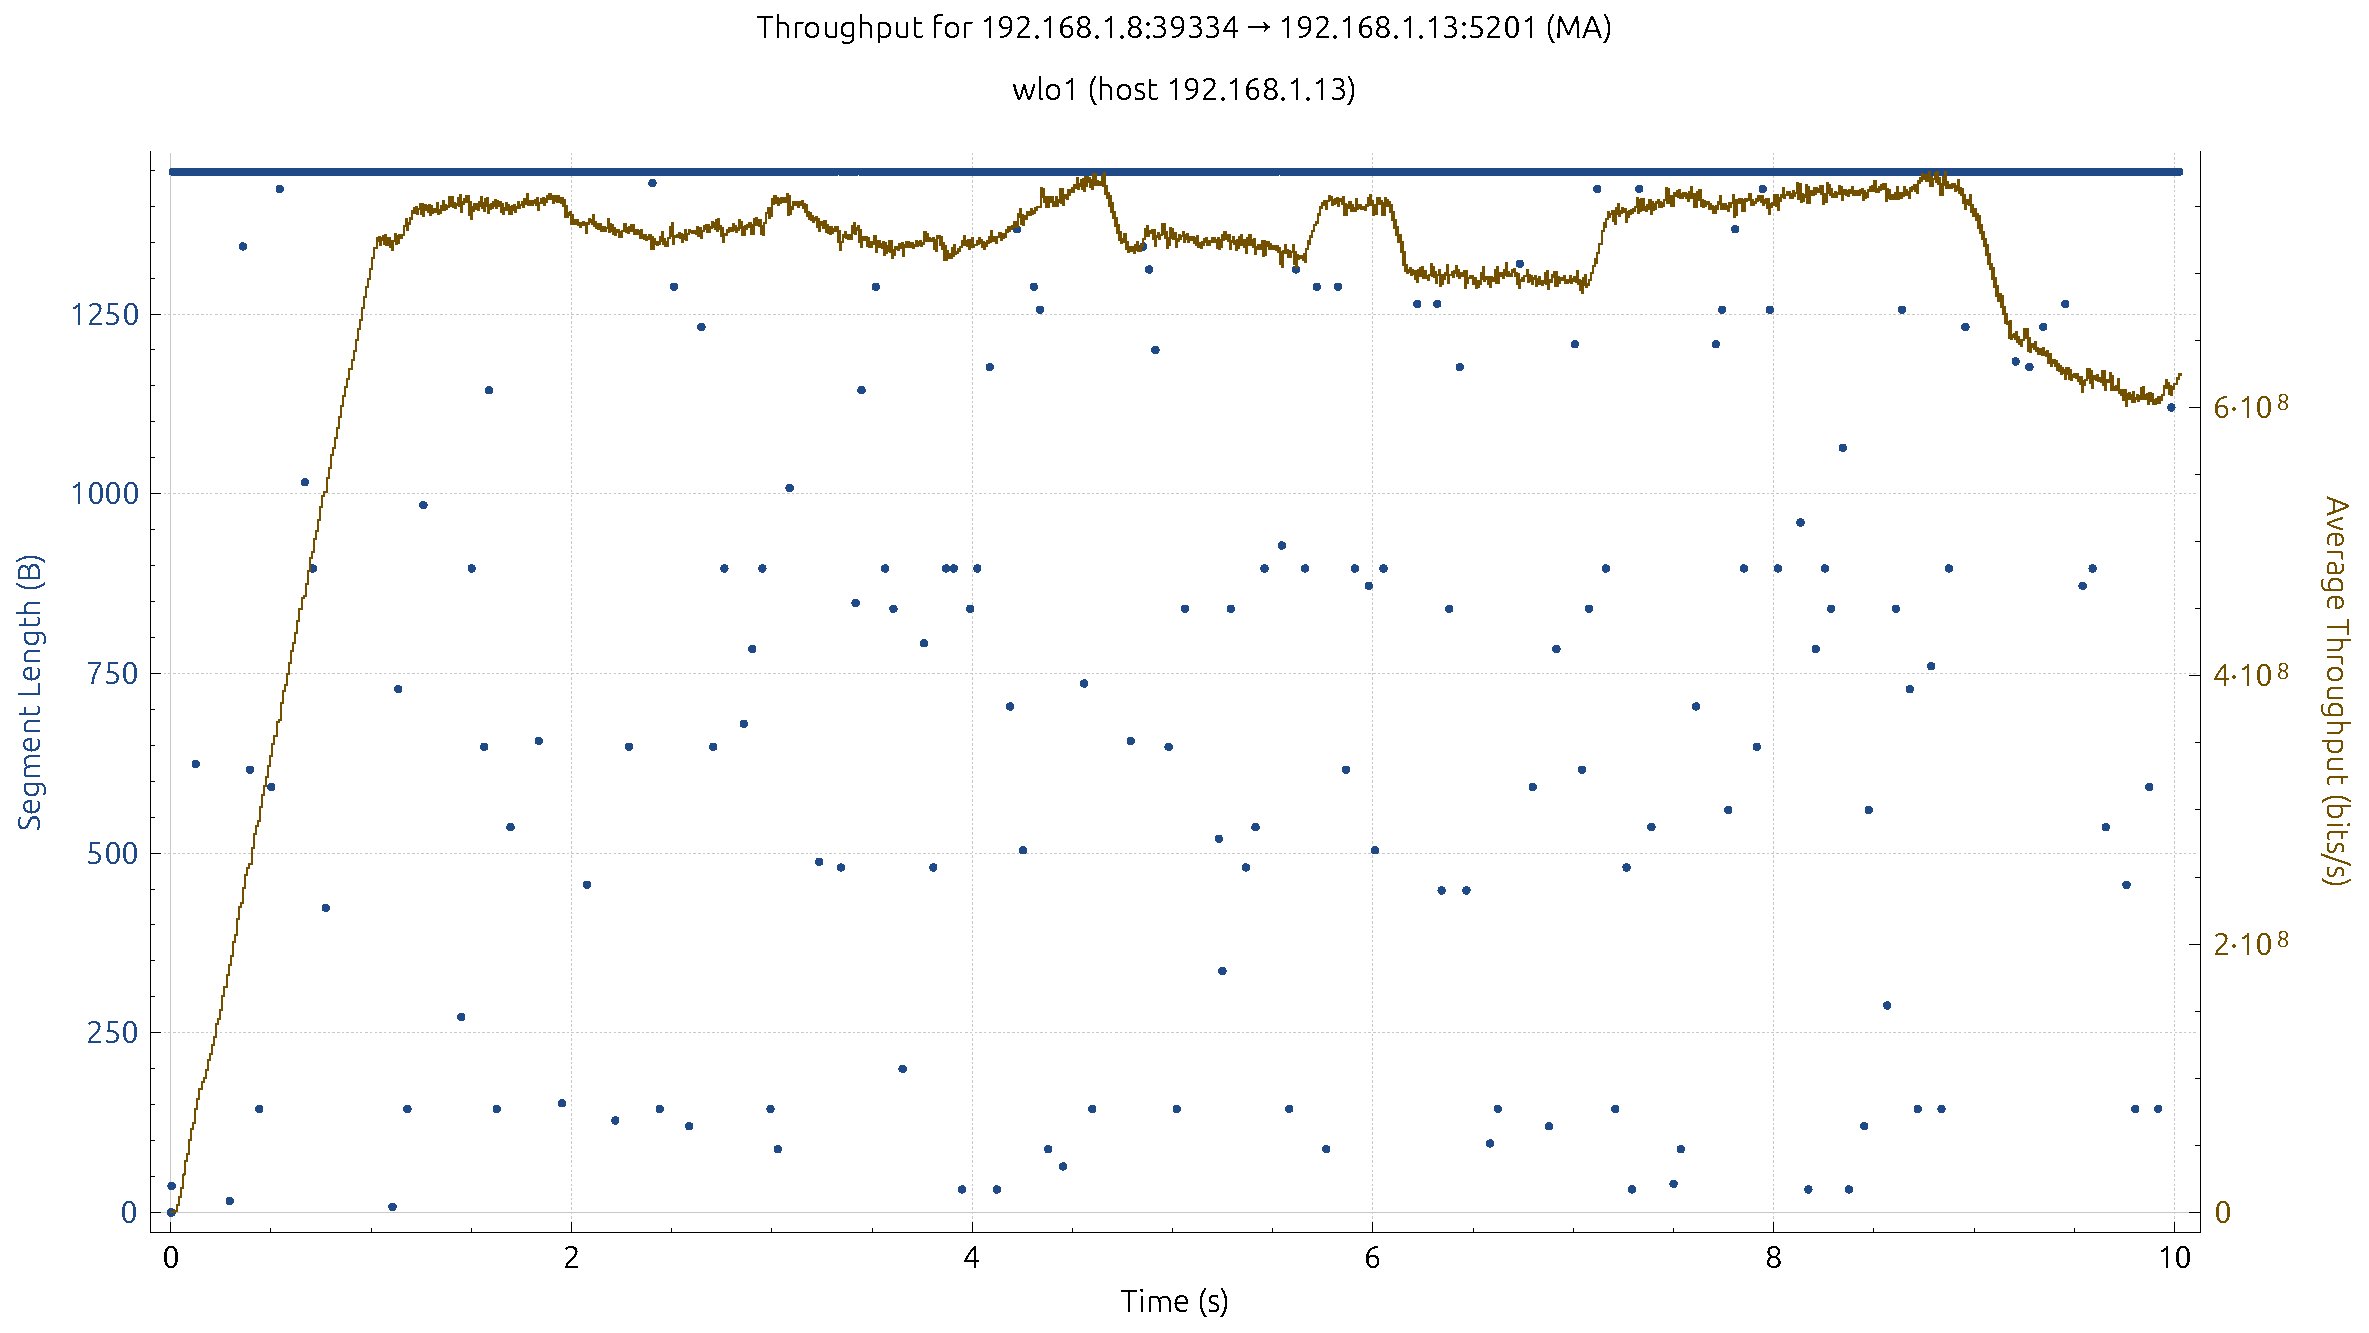
\includegraphics[width=0.9\columnwidth]{images/graphs/Throughput/Throughput_MIX_MITM_TCP.pdf}
                %     \caption{TCP Throughput in the Shared Capacity Scenario (with third-host interference).}
                %     \label{fig:throughput-mitm-tcp}
                % \end{figure}

                % The round-trip time measurements (Fig.~\ref{fig:rtt-mitm-tcp}) indicate increased variability and slightly elevated latency. 
                % Although the RTT values remain relatively moderate, the fluctuations suggest that the network experiences occasional congestion and delays as a result of the third host's activity.

                % \begin{figure}[ht]
                %     \centering
                %     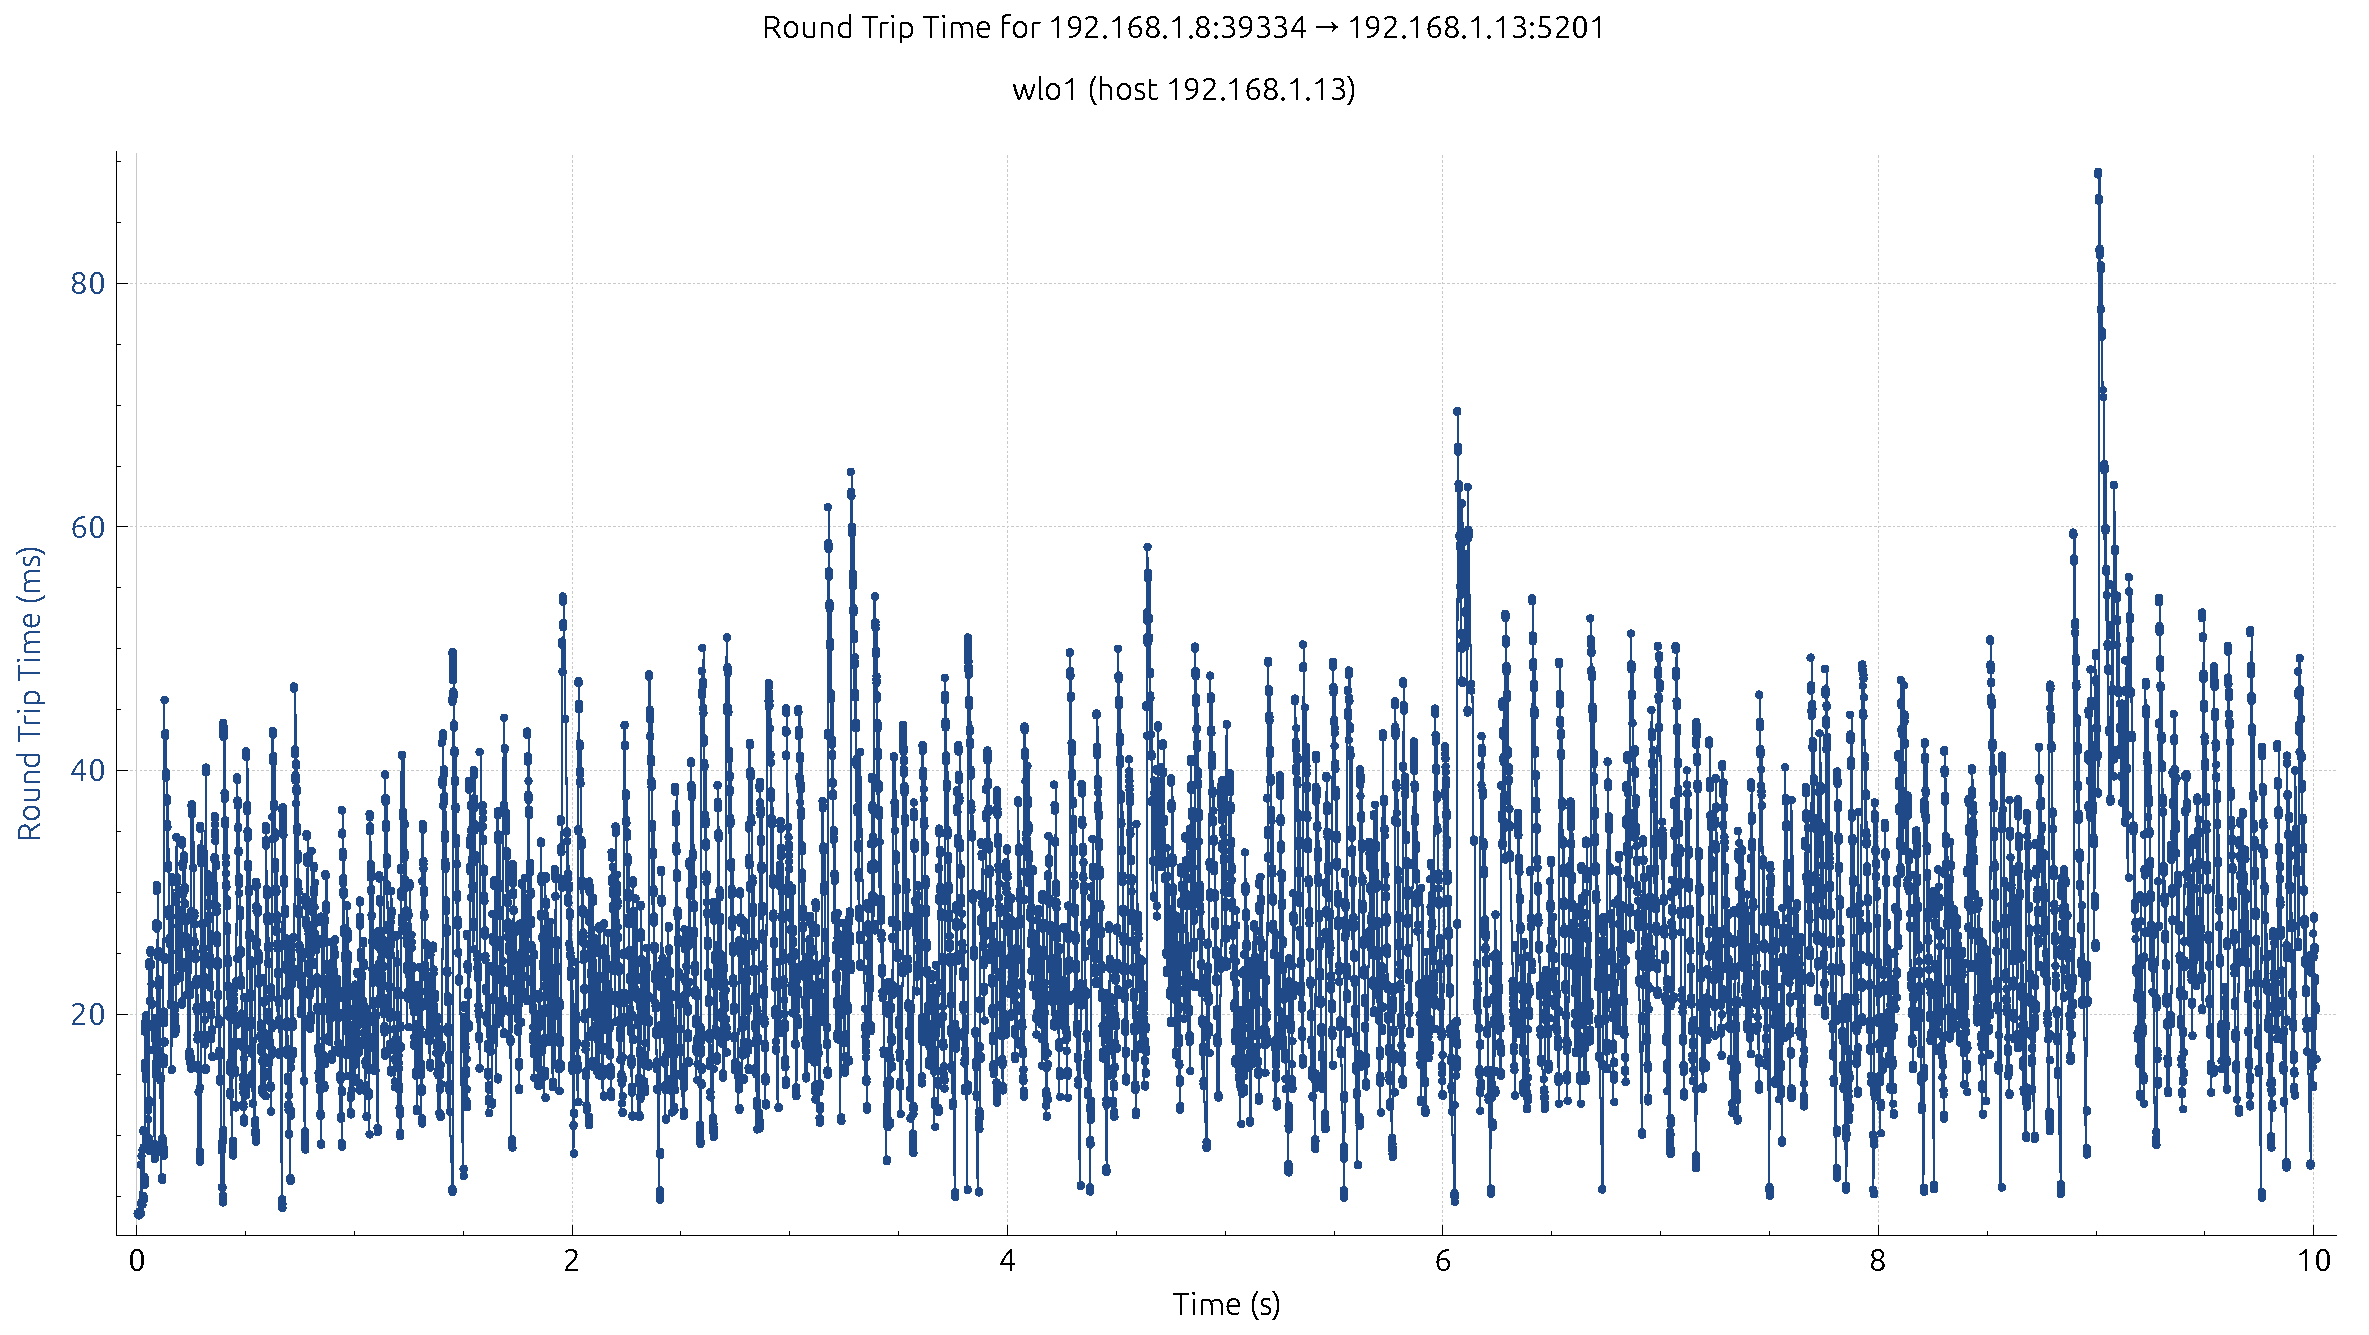
\includegraphics[width=0.9\columnwidth]{images/graphs/RTT/RTT_MIX_MITM_TCP.pdf}
                %     \caption{TCP Round Trip Time in the Shared Capacity Scenario.}
                %     \label{fig:rtt-mitm-tcp}
                % \end{figure}

                % The I-O graph for TCP (Fig.~\ref{fig:io-mitm-tcp}) further confirms the impact of the interference. 
                % The graph displays irregular intervals and a lower packet transmission rate compared to the mixed scenario without the additional load, demonstrating how the extra traffic disrupts the steady flow of data.

                \begin{figure}[ht]
                    \centering
                    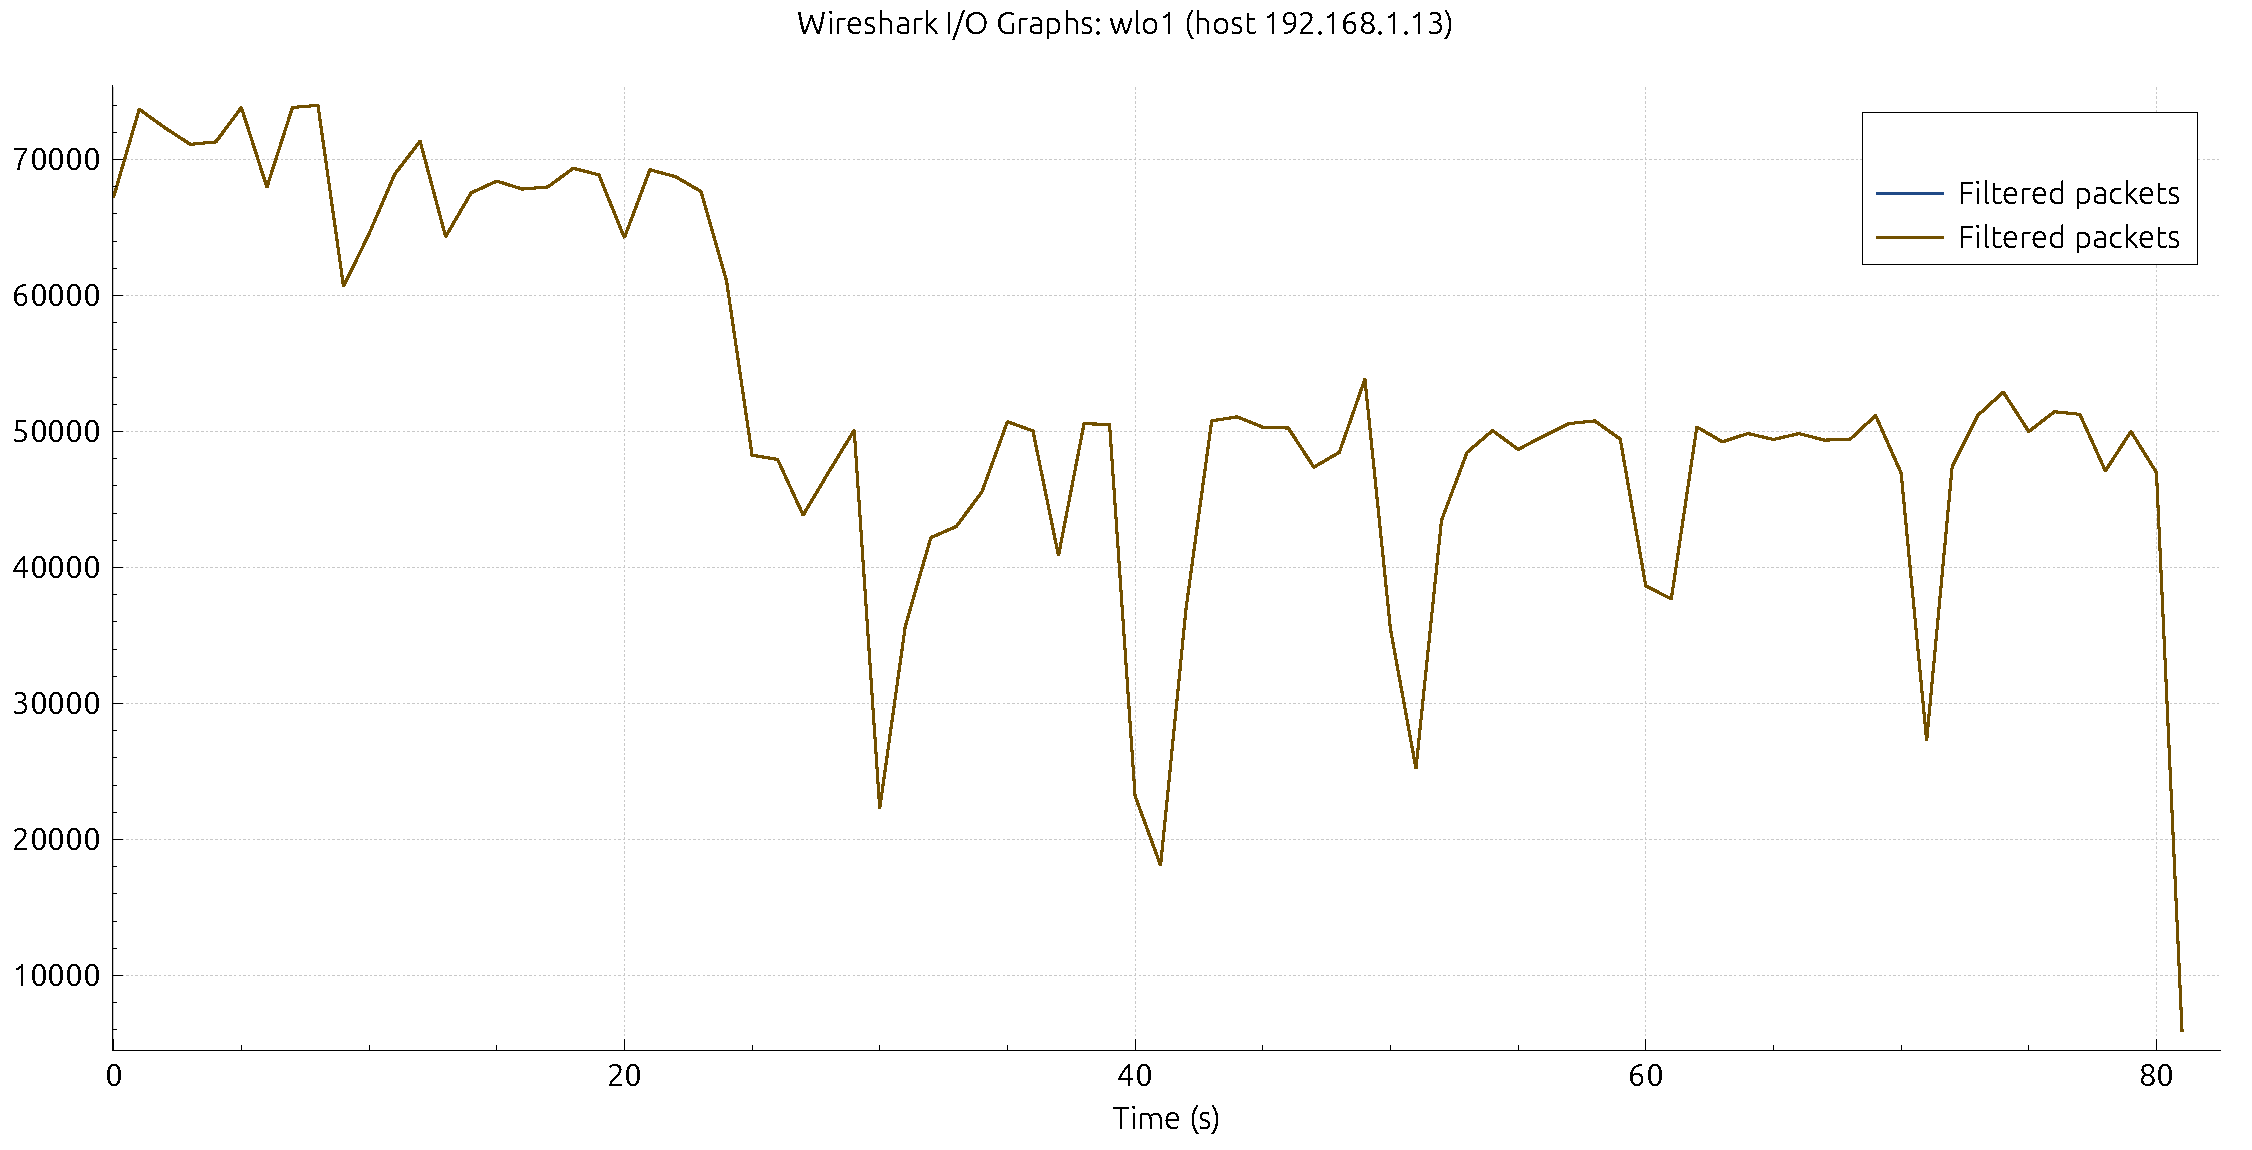
\includegraphics[width=0.9\columnwidth]{images/graphs/I-O/I-O_MIX_MITM_TCP.pdf}
                    \caption{Wireshark I-O Graph for TCP in the Shared Capacity Scenario.}
                    \label{fig:io-mitm-tcp}
                \end{figure}

        \end{enumerate}

    \subsection{UDP Performance} \label{subsec:udp-performance}

        The UDP tests offer an insightful comparison to the TCP results by eliminating congestion control and acknowledgment overhead. The analysis for UDP is structured as follows:

        \begin{table}[H]
            \small
            \centering
            \begin{tabular}{|ll|lllll|}
            \hline
            % \multicolumn{2}{|c|}{\multirow{2}{*}{\makecell{\textbf{Test} \\ Client $\rightarrow$ Server}}} & 
            \multicolumn{2}{|c|}{\multirow{2}{*}{\textbf{Test}}} & 
                \multicolumn{5}{c|}{\textbf{UDP: Goodput per flow (Mbps)}} \\
            \cline{3-7}
            \multicolumn{2}{|c|}{} &
                \multicolumn{1}{c|}{Prediction} &
                \multicolumn{1}{c|}{Average} &
                \multicolumn{1}{c|}{Min} &
                \multicolumn{1}{c|}{Max} &
                \multicolumn{1}{c|}{Std} \\
            \hline
            \multicolumn{2}{|c|}{Both Ethernet} &
                \multicolumn{1}{c|}{957} &
                \multicolumn{1}{c|}{952.8} &
                \multicolumn{1}{c|}{948.3} &
                \multicolumn{1}{c|}{954.6} &
                \multicolumn{1}{c|}{1.73} \\
            \hline
            \multicolumn{2}{|c|}{Both WiFi} &
                \multicolumn{1}{c|}{510} &
                \multicolumn{1}{c|}{487.8} &
                \multicolumn{1}{c|}{453.1} &
                \multicolumn{1}{c|}{499.9} &
                \multicolumn{1}{c|}{15.8} \\
            \hline
            \multicolumn{2}{|c|}{Mixed} &
                \multicolumn{1}{c|}{957} &
                \multicolumn{1}{c|}{674.9} &
                \multicolumn{1}{c|}{636.6} &
                \multicolumn{1}{c|}{717.8} &
                \multicolumn{1}{c|}{28} \\
            \hline
           % \multicolumn{2}{|c|}{Shared Capacity} &
           %     \multicolumn{1}{c|}{?} &
           %     \multicolumn{1}{c|}{472.1} &
           %     \multicolumn{1}{c|}{355.9} &
           %     \multicolumn{1}{c|}{699.1} &
           %     \multicolumn{1}{c|}{121.1} \\
           % \hline
            \end{tabular}
            \vspace{0.5cm}
            \caption{UDP Results (Client $\rightarrow$ Server)}
            \label{tab:udp-results}
        \end{table}

        \vspace{-0.3cm}

        \begin{enumerate}
            \item \textbf{Both Ethernet:} \\
                In the Ethernet scenario, UDP achieves a near-theoretical throughput of \textbf{952.8 Mbps} (vs. TCP’s 939.6 Mbps), with minimal standard deviation (\textbf{1.73 Mbps}). The absence of retransmissions or congestion control allows UDP to utilize the full wired capacity. While TCP’s latency remains marginally lower (1–3 ms RTT) due to acknowledgment-based stability, UDP’s lack of overhead enables slightly higher throughput.
            \\

            \item \textbf{Both WiFi:} \\
            UDP averages \textbf{487.8 Mbps} (vs. TCP’s 434.7 Mbps) in WiFi, achieving a \textbf{\textasciitilde 12\% throughput advantage} by avoiding TCP’s congestion control. Despite outperforming TCP, UDP falls short of the \textbf{510 Mbps theoretical maximum} due to WiFi interference and contention. Moreover, it shows lower variability (std. dev. \textbf{15.8 Mbps} vs. TCP’s \textbf{22.5 Mbps}), indicating smoother performance. This makes UDP preferable for real-time applications prioritizing speed over error correction.
            \\

            \item \textbf{Mixed:} \\
                In the mixed configuration, UDP achieves an average throughput of \textbf{674.9 Mbps}, marginally higher than TCP but still far below the theoretical \textbf{957 Mbps}. While UDP bypasses TCP’s RTT-dependent limitations, the wireless link’s inherent instability, evident in its higher standard deviation (28 Mbps vs. Ethernet’s 1.73 Mbps), remains the dominant bottleneck, highlighting that protocol-agnostic medium constraints govern hybrid network performance
            \\

            \item[3a.] \textbf{Shared Capacity:} \\
                In the shared capacity test, UDP throughput drops significantly. The third host’s download introduces contention, reducing available bandwidth. UDP’s lack of congestion control leads to aggressive transmission attempts, but packet drops result in lower effective throughput. Unlike TCP, which degrades predictably due to its back-off mechanism, UDP’s performance becomes more volatile. This highlights TCP’s adaptability in shared environments, where fairness and resource allocation are critical, while UDP’s rigidity makes it less suitable for contested networks.
        \end{enumerate}
    